\chapter{Desenvolvimento}
  
\section{O funcionamento do termistor}
 
	O termistor é um resistor variável à temperatura, característica pela qual seu nome é inspirado (temperatura + resistor), geralmente compostos por uma liga que contém cerâmica e outros polímeros. Suas aplicações mais habituais costumam acontecer em circuitos de monitoramento e controle de temperatura ou como limitador de corrente de partida. São separados, basicamente, em duas categorias:
	\begin{itemize}
		\item NTC (Negative Temperature Coefficient): São termistores que diminuem a sua resistência à medida em que a temperatura aumenta; E
		\item PTC (Positive Temperature Coefficient): Termistores que aumentam a sua resistência diretamente com o aumento da temperatura.
	\end{itemize}
	
	\subsection{A equação de Steinhart–Hart}
	
		A curva de variação da resistência de um termistor em função de sua temperatura pode ser descrita pela equação de Steinhart–Hart\ref{eq:steinharthart} em sua forma inversa \ref{eq:steinharthartinverted}. A característica logarítmica da resposta com que a resistência varia em função da variação de temperatura (figura \ref{fig:curva_termistor}) é, em grande parte das vezes, uma das principais vantagens do seu uso, visto que pequenas variações na temperatura provocam grandes alterações na resistência, fazendo com que o sensor seja mais suscetível a detectar pequenas mudanças na temperatura.
		
		
		\begin{equation}\label{eq:steinharthart}
		\dfrac{1}{T} = a + b\ln{(R)} + c(\ln{(R)})^3
		\end{equation}
		Sendo:
		\begin{itemize}
			\item T: Temperatura em Kelvins;
			\item R: Resistência em ohms ($\Omega$);E
			\item a,b e c: Coeficientes de Steinhart–Hart, que são variáveis conforme o tipo de material e a construção do termistor.		
		\end{itemize}
		
		
		\begin{equation}\label{eq:steinharthartinverted}
			\begin{aligned} [left]
			& R = \exp{(\sqrt[3]{\beta - \dfrac{\alpha}{2}} - \sqrt[3]{\beta + \dfrac{\alpha}{2}})},
			\\
			& \alpha = \dfrac{1}{c}(a - \dfrac{1}{T}),
			\\
			& \beta = \sqrt{(\dfrac{b}{3c})^3 + (\dfrac{\alpha}{2})^2}
			\end{aligned}
		\end{equation}
	
	
		\begin{figure}[h!]
			\begin{center}
				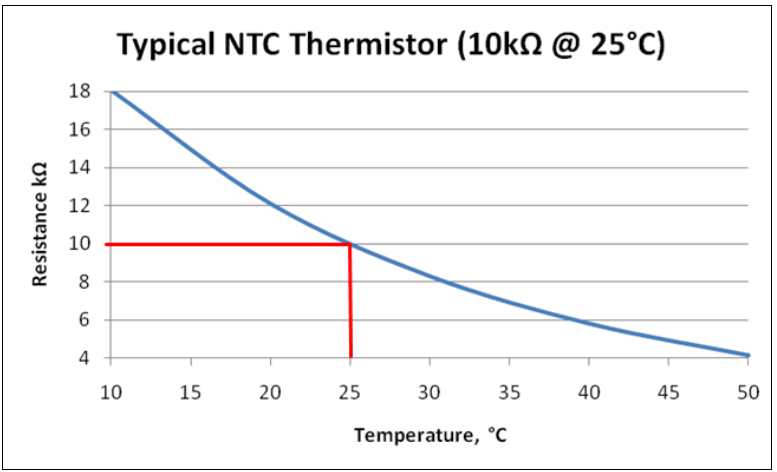
\includegraphics[width=1\linewidth]{images/curva_termistor.png}
				\caption[Curva de resposta típica em termistores NTC de 10k$\Omega$]{Curva de resposta típica em termistores NTC de 10k$\Omega$\footnotemark}
				\label{fig:curva_termistor}
			\end{center}
		\end{figure}
	
		\footnotetext{Fonte: http://www.squids.com.br/arduino/index.php/projetos-arduino/projetos-squids/basico/159-projeto-42-comparando-sensores-de-temperatura-ntc-10k-dht11-e-lm35}


	\subsection{O efeito de Autoaquecimento}

		Como toda resistência, o termistor dissipa energia elétrica na forma de calor. Portanto, ao aplicar uma corrente no sensor, é induzido um efeito de autoaquecimento. A relação da potência elétrica dissipada é dada pela equação \ref{eq:potenciaeletrica} e a relação entre potência e temperatura pode ser obtida através da equação \ref{eq:potenciatermica}. Fazendo $P_E = P_T$, é possível chegar à equação \ref{eq:temperaturacomautoaquecimento}. 
		
		\begin{equation}\label{eq:potenciaeletrica}
			P_E = I.V
		\end{equation}
		sendo:
		\begin{itemize}
			\item $P_E$: Potência elétrica dissipada;
			\item $I$: Corrente elétrica;E
			\item $V$: Tensão entre os terminais.
		\end{itemize}

		\begin{equation}\label{eq:potenciatermica}
			P_T = K(T_{(R)} - T_0)
		\end{equation}
		sendo:
		\begin{itemize}
			\item $P_T$: Potência;
			\item $K$: Fator de dissipação do termistor;
			\item $T_{(R)}$: Temperatura em função da resistência;E
			\item $T_0$: Temperatura ao redor do termistor.
		\end{itemize}
		
		\begin{equation} \label{eq:temperaturacomautoaquecimento}
			T_0 = T_{(R)} - \dfrac{V^2}{K.R}
		\end{equation}
		

\section{A evolução do circuito}

\subsection{O divisor resistivo}

A priori, a medição da frequência respiratória seria obtida indiretamente pela variação da temperatura do ar próximo à narina do paciente, uma vez que, em um ambiente controlado, o ar inalado possui uma temperatura inferior à do ar exalado. Valendo-se da propriedade logarítmica do termistor, uma pequena variação de temperatura ambiente ocasionada pelo processo de expiração ocasionaria uma mudança exponencial no valor da resistência. Por esse motivo, na origem do projeto, era esperada uma medição simples, obtida através da variação de tensão em um divisor resistivo composto por um termistor e uma resistência padrão(Figura: \ref{fig:divisorResistivo}).
 
Foi construído o primeiro divisor resistivo apenas com base na informação de que o sensor adquirido tratava-se de um termistor NTC (do inglês Negative Temperature Coefficient) com resistência em temperatura ambiente de $10K\Omega$, sem acesso ao datasheet do componente. Foi utilizada uma fonte de alimentação comercial de $12V$ e utilizado diversos valores entre $10K\Omega$ e $330\Omega$ para a resistência $R2$, contudo para nenhum valor de $R2$ era observada qualquer alteração de tensão na medida em que o ar era exalado próximo ao sensor, contrariando ao que era esperado, dado que a queda de tensão em cima do termistor deve ser variável junto à alteração na resistência.
 
\begin{figure}[h!]
	\begin{center}
 		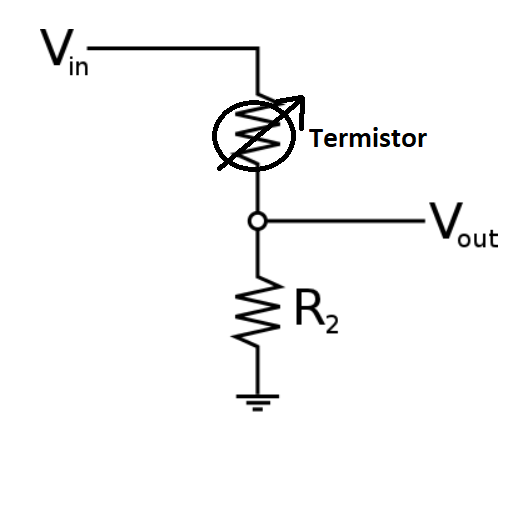
\includegraphics[width=0.5\linewidth]{images/divisor_resistivo.png}
 		\caption{Divisor Resistivo}
 		\label{fig:divisorResistivo}
 	\end{center}
\end{figure}
 
\subsection{Lei de resfriamento de Newton} \label{sec:lei_de_resfriamento}
 
A lei de resfriamento de Newton (\ref{eq:resfriamento}) indica que a taxa com que um corpo perde calor é proporcional à diferença de temperatura entre o corpo e o meio  no qual ele se encontra. Valendo-se desse princípio, nota-se que uma baixa diferença de temperatura resultaria em um maior tempo de resposta do sensor. 
 
  
\begin{equation} \label{eq:resfriamento}
	\dfrac{dQ}{dt} = h.A.(T(t) - T_{env}) = h.A \Delta T(t)	
\end{equation}
Onde:
\begin{itemize}[label=]
	\item $Q$: Energia térmica
	\item $t$: Tempo
	\item $h$: Coeficiente de transferência de calor
	\item $A$: Área de transferência de calor
	\item $T$: Temperatura do objeto
	\item $T_{env}$: Temperatura do ambiente
\end{itemize}
 
\begin{equation} \label{eq:autoAquecimento}
	T_0 = T(R) - \dfrac{V^2}{KR}
\end{equation}
Onde:
\begin{itemize}[label=]
	\item $T_0$: Temperatura do meio
 	\item $T(R)$: Temperatura do termistor em função de sua resistência
 	\item $V$: Diferença de potencial entre os terminais do termistor
 	\item $K$: Fator de dissipação do termistor
 	\item $R$: Resistência
\end{itemize}
 

\subsection{Circuito utilizando o efeito do autoaquecimento}

Em decorrência da lei de resfriamento de Newton \ref{sec:lei_de_resfriamento} e considerando a baixa variação de temperatura para esse tipo de medição, seria inviável a realização da medida diretamente pela diferença de temperatura entre inspiração e expiração, dada a velocidade de resposta necessária para a obtenção dos dados de forma confiável e a utilização de equipamentos de baixo custo como requisito. Para contornar esse problema, foi utilizada a propriedade de autoaquecimento do termistor (\ref{eq:autoAquecimento}), que passou a ser utilizado como um sensor de fluxo. Ou seja, o sistema não mais tenta inferir a frequência respiratória com base no aumento da temperatura ambiente ocasionada pela saída de ar quente do corpo humano, ao contrário, ele aplica uma corrente muito alta no sensor forçando-o a atingir por conta própria uma temperatura ainda maior em seu estado permanente e, no momento de seu encontro com qualquer fluxo de ar resultante da respiração humana, o sensor registra uma alta queda de temperatura, registrando, de forma mais nítida o momento da ação respiratória.

Ao aplicar uma alta corrente no sensor, é induzido então um aumento na temperatura deste. Em decorrência desse aumento, é possível observar uma maior diferença de temperatura entre o sensor e o fluxo de ar e, por conseguinte, uma maior taxa para transferência de calor e um menor tempo de resposta por parte do termistor. Contudo, para atingir uma faixa de temperatura sensível, capaz de gerar uma resposta visível ao expor o sensor à respiração, o circuito necessita de uma tensão elevada, acima das entregues por fontes comerciais padrão, que costumam variar entre $5V$ e $12V$, gerando a necessidade de projetar um retificador de tensão capaz de converter a tensão de corrente alternada entregue pela rede elétrica residencial em uma tensão contínua alta o suficiente para fornecer ao termistor a corrente demandada.
 
Realizando testes de bancada, com um gerador de tensão variando de $0V$ à $30V$ e uma resistência de $330\Omega$ em série com o termistor, foi possível atingir uma temperatura sensível ao sopro, entretanto, ao aplicar uma tensão em torno de $22V$, o sensor demorava um tempo considerável para aquecer novamente, tornando-o inviável para medir o comportamento respiratório dada a frequência do sopro em uma respiração normal. Aumentando a tensão para $28V$, já era possível observar uma atenuação considerável na queda constante da temperatura dado que o termistor era capaz de se aquecer mais rápido. O problema gerado por esse aumento de tensão deve-se ao fato de que, quanto maior é a corrente, maior é o autoaquecimento e, quanto maior a temperatura, menor é a resistência, gerando um aumento ainda maior na corrente passante que, por sua vez, aumenta ainda mais a temperatura até que o sensor atingia um patamar no qual queimava, caso não houvesse nenhum sopro forçando a temperatura a diminuir. 
 
Para suprir o fornecimento de tensão em corrente contínua em torno dos $28V$ foi necessário construir um retificador de tensão, uma vez que as fontes padrão, encontradas no mercado, costumam fornecer tensão menor que a desejada. O circuito projetado para a fonte de corrente encontra-se na figura \ref{fig:circuito_retificador}.

\begin{figure}[h!]
	\begin{center}
		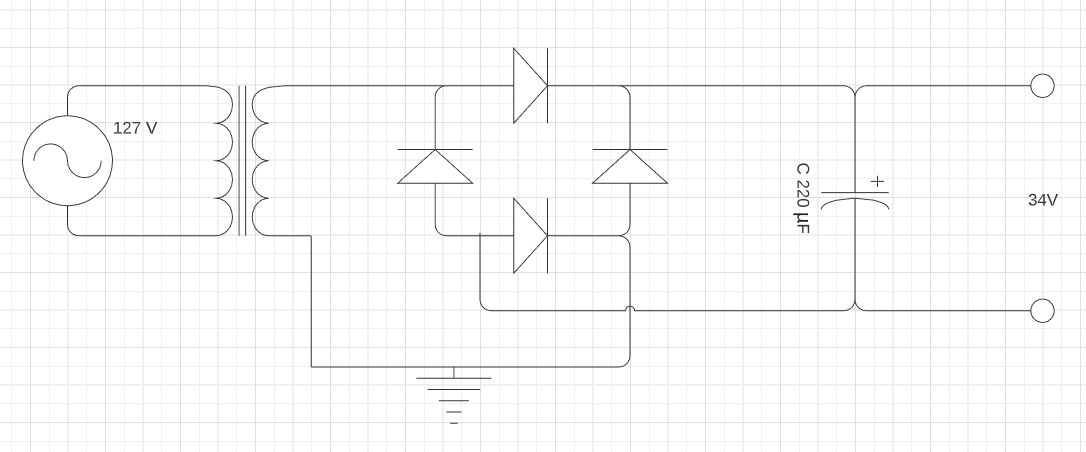
\includegraphics[width=1\linewidth]{images/circuito_retificador.png}
		\caption{Retificador de Tensão}
		\label{fig:circuito_retificador}
	\end{center}
\end{figure} 
 
 
\subsection{Circuito com controle realimentado} 
 
Se por um lado, o aumento da tensão era importante para que a temperatura não decaísse constantemente ao iniciar a medição respiratória, por outro, o sistema precisava ser protegido para que a corrente não atingisse um determinado patamar que danificasse o componente. O ajuste mais simples para regular a corrente em um componente costuma ser adicionar uma resistência em série, diminuindo a corrente por uma mera consequência da lei de ohm (\ref{eq:leideohm}). Contudo, por se tratar de uma resistência variável, a tensão necessária para o aquecimento do termistor em seu estado inicial era maior que a tensão necessária para mantê-lo abaixo de um patamar seguro após a diminuição de sua resistência pelo efeito do autoaquecimento. Foi desenvolvido então em um circuito de controle não linear (Figura: \ref{fig:circuitoRealimentado}), que, em teoria, forneceria uma alta tensão para o termistor até que sua resistência variasse e a corrente passante atingisse um patamar determinado. O comportamento esperado para o circuito de controle seria o seguinte: 

\begin{itemize}
	\item [1-] O amplificador operacional iria ajustar a tensão de saída na tentativa de igualar as tensões nos dois terminais de entrada.
	\item [2-] Quando a tensão no terminal de entrada negativo é igual a zero e a do terminal positivo é igual a $5V$, o amplificador aumenta sua saída fazendo com que o transistor entre em saturação e conduza uma corrente no emissor praticamente igual à de referência no coletor.
	\item [3-] Na medida em que a resistência do termistor diminui pelo efeito de autoaquecimento, a tensão de saída aumenta até que esta se iguale à do terminal positivo.
	\item [4-] Após igualar a tensão nos terminais do amplificador, o transistor sai da zona de saturação e o sistema trabalha pra manter a tensão de saída constante.
	\item [5-] No momento em que o sensor entra em contato com o fluxo de ar, a resistência do termistor aumenta, diminuindo a tensão na saída e estimulando o sistema de controle a saturar o transistor e induzir o efeito do autoaquecimento no sensor. 
\end{itemize}

\begin{figure}[h!]
	\begin{center}
		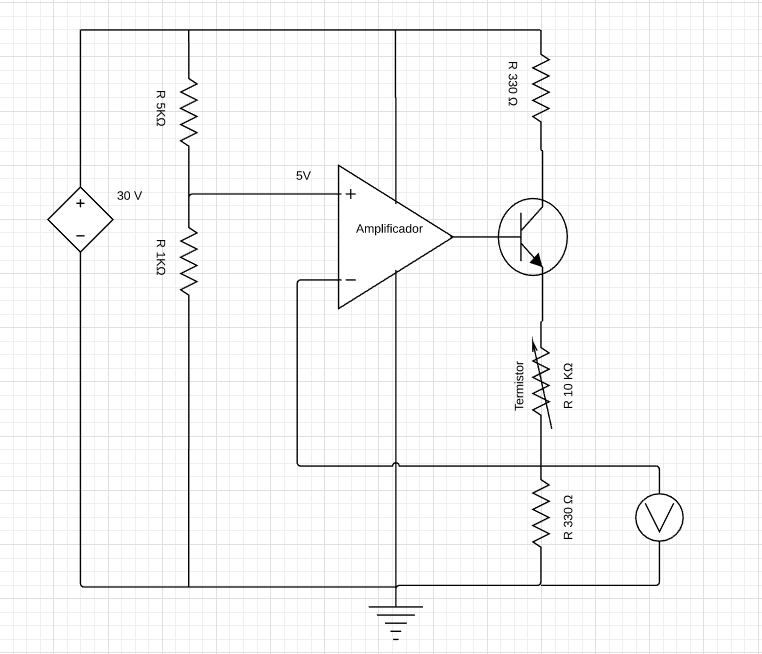
\includegraphics[width=1\linewidth]{images/Circuito_de_controle.png}
		\caption{Circuito de Controle}
		\label{fig:circuitoRealimentado}
	\end{center}
\end{figure}
\FloatBarrier

\begin{equation} \label{eq:leideohm}
V = R.I
\end{equation}
Onde:
\begin{itemize}[label=]
	\item $V$: Tensão
	\item $R$: Resistência
	\item $I$: Corrente
\end{itemize}

\section{Resultados e medições do hardware}

\subsection{Medição da variação do Termistor}

Para entender melhor o comportamento do termistor e a forma com que ele variava sua resistência devido o efeito do autoaquecimento, sem acesso ao datasheet do mesmo, foram realizadas medições utilizando o divisor resistivo, colocando o termistor em série com um resistor fixo de $330\Omega$ e uma fonte de bancada com fornecimento de tensão variável entre $0V$ e $30V$. A curva de variação pode ser observada no gráfico da figura \ref{fig:variacao_termistor}.

\begin{figure}[h!]
	\begin{center}
		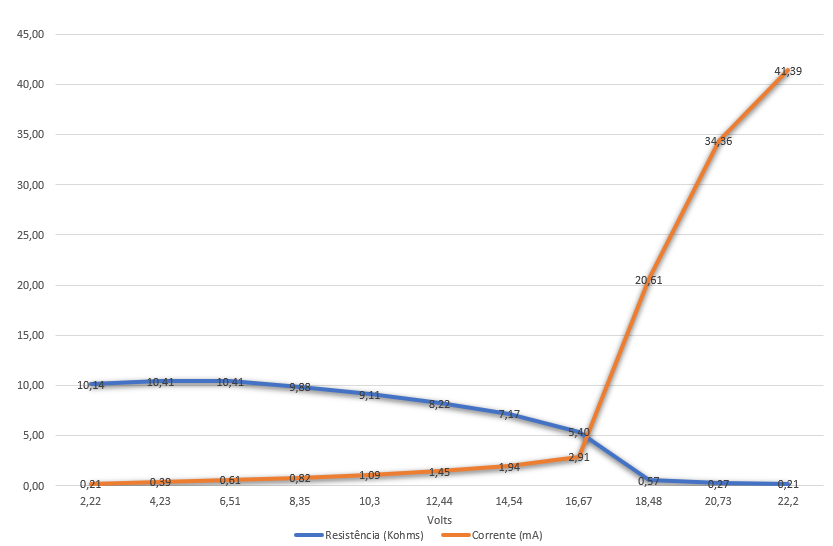
\includegraphics[width=0.9\linewidth]{images/variacao_resistencia_termistor.png}
		\caption{Variação do termistor em função da tensão}
		\label{fig:variacao_termistor}
	\end{center}
\end{figure}
\FloatBarrier

\subsection{Fonte de tensão}

Para entregar a tensão necessária ao circuito foi construído o retificador da foto \ref{fig:fonte_circuito}, capaz de entregar uma tensão de saída na ordem de $34V$ conforme a medida \ref{fig:fonte_medicao}

\begin{figure}[h!]
	\begin{center}
		\includegraphics[width=0.5\linewidth]{images/fonte_circuito.jpg}
		\caption{Retificador de tensão}
		\label{fig:fonte_circuito}
	\end{center}
\end{figure}

\begin{figure}[h!]
	\begin{center}
		\includegraphics[width=0.5\linewidth]{images/fonte_medicao.jpg}
		\caption{Medição da tensão de saída do retificador}
		\label{fig:fonte_medicao}
	\end{center}
\end{figure}
\FloatBarrier

\subsection{Máscara respiratória}

Para acomodar o sensor e forçar o contato do fluxo de ar, tanto da expiração quanto da inspiração, em sua superfície, foi adaptada uma máscara de nebulização. A saída de ar foi vedada com fita isolante, o sensor alocado em sua parte inferior e pequenos furos foram realizados por onde ocorrerá a troca de ar com o meio externo. O protótipo pode ser observado nas figuras \ref{fig:mascara1}, \ref{fig:mascara2} e \ref{fig:mascara3}.

\begin{figure}[h!]
	\begin{center}
		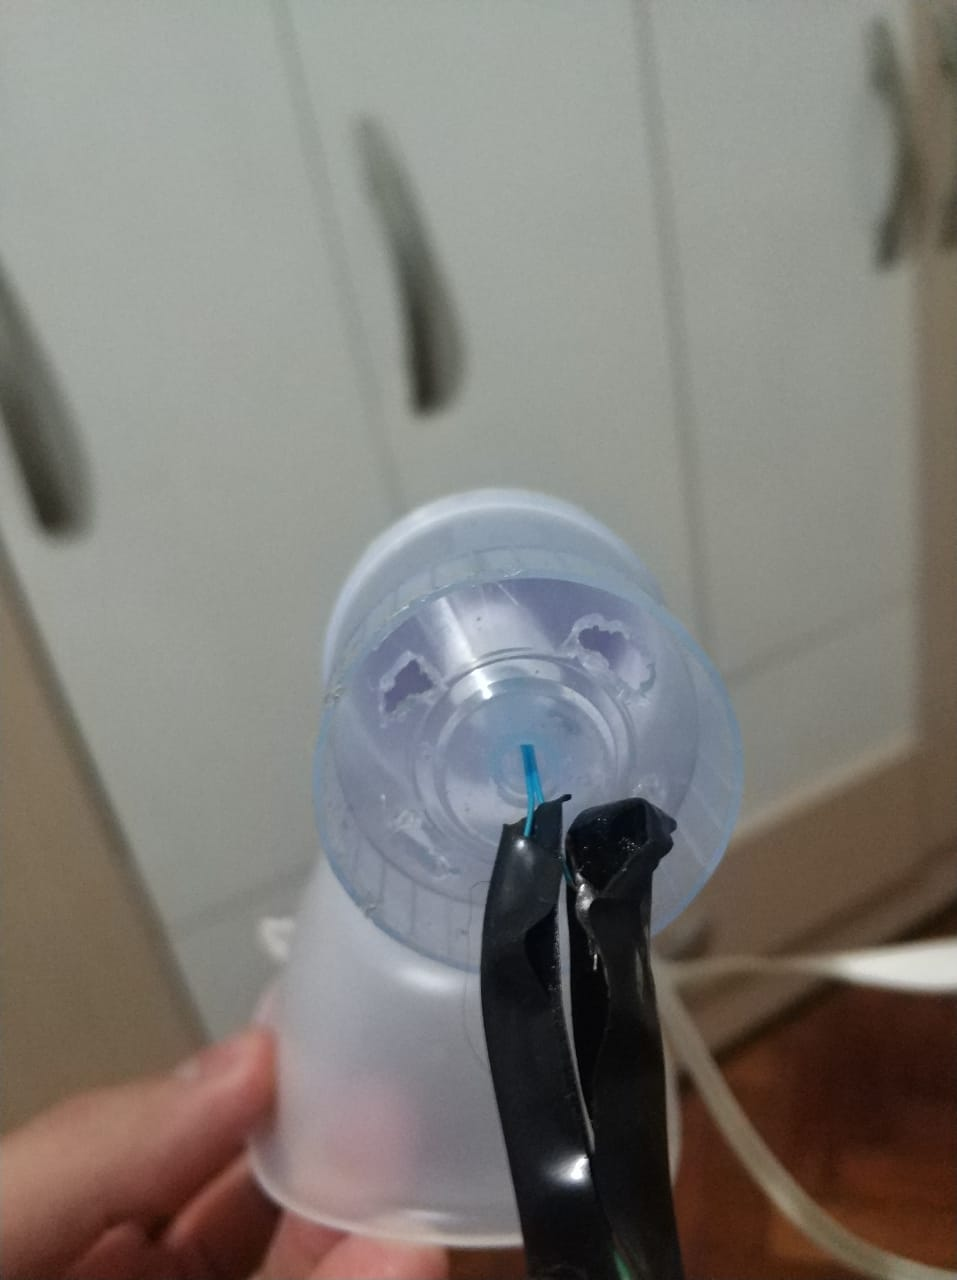
\includegraphics[width=0.5\linewidth]{images/mascara1.jpeg}
		\caption{Máscara respiratória}
		\label{fig:mascara1}
	\end{center}
\end{figure}

\begin{figure}[h!]
	\begin{center}
		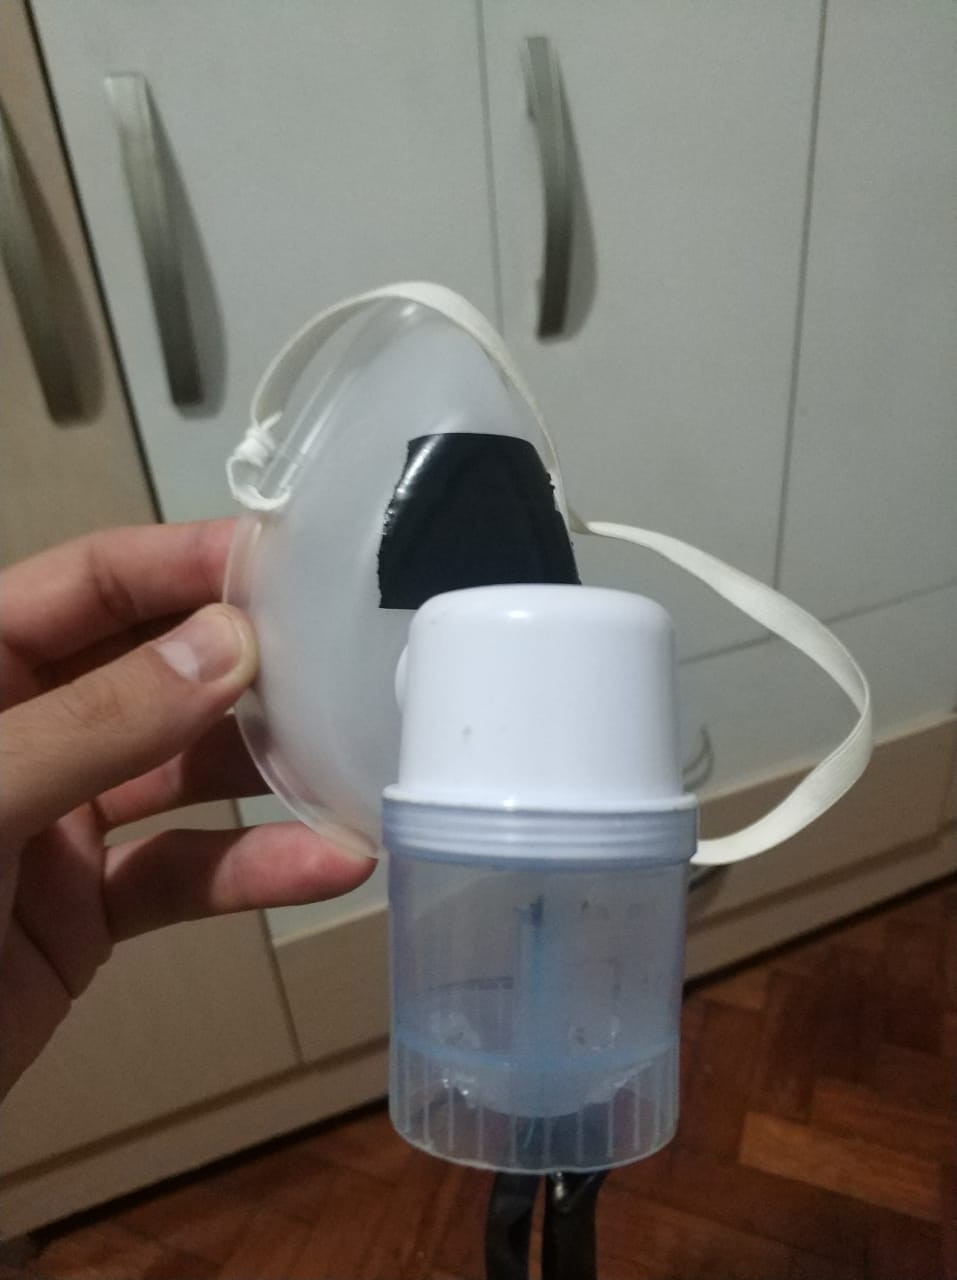
\includegraphics[width=0.8\linewidth]{images/mascara2.jpeg}
		\caption{Máscara respiratória}
		\label{fig:mascara2}
	\end{center}
\end{figure}

\begin{figure}[h!]
	\begin{center}
		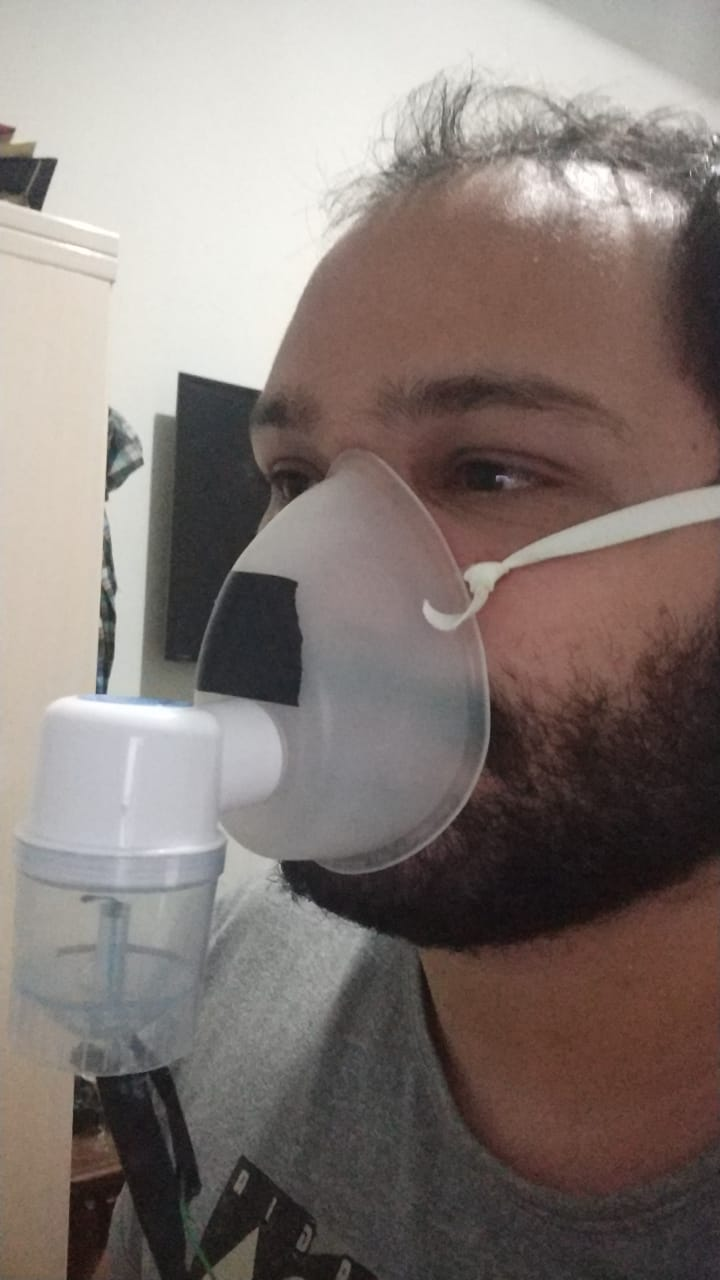
\includegraphics[width=0.8\linewidth]{images/mascara3.jpeg}
		\caption{Máscara respiratória}
		\label{fig:mascara3}
	\end{center}
\end{figure}
\FloatBarrier

\subsection{Teste do circuito realimentado}

Após realizar uma medição respiratória de teste e quantizar a tensão da saída através de um microcontrolador, foi possível traçar o gráfico da figura \ref{fig:RespostaCircuitoRealimentado}, no qual aparece nítida a resposta do sistema ao submeter o sensor a um fluxo de ar. Entretanto, ao expor o sensor a um período prolongado de exposição à respiração humana, foi possível observar que o efeito do resfriamento contínuo continuava a ser reproduzido (gráfico da figura \ref{fig:RespostaCircuitoRealimentadoLongoPrazo}). Ao analisar o sinal em um osciloscópio com filtro AC, conseguimos ter o sinal em sua melhor forma, conforme a figura \ref{sinal_osciloscopio}.


\begin{figure}[h!]
	\begin{center}
		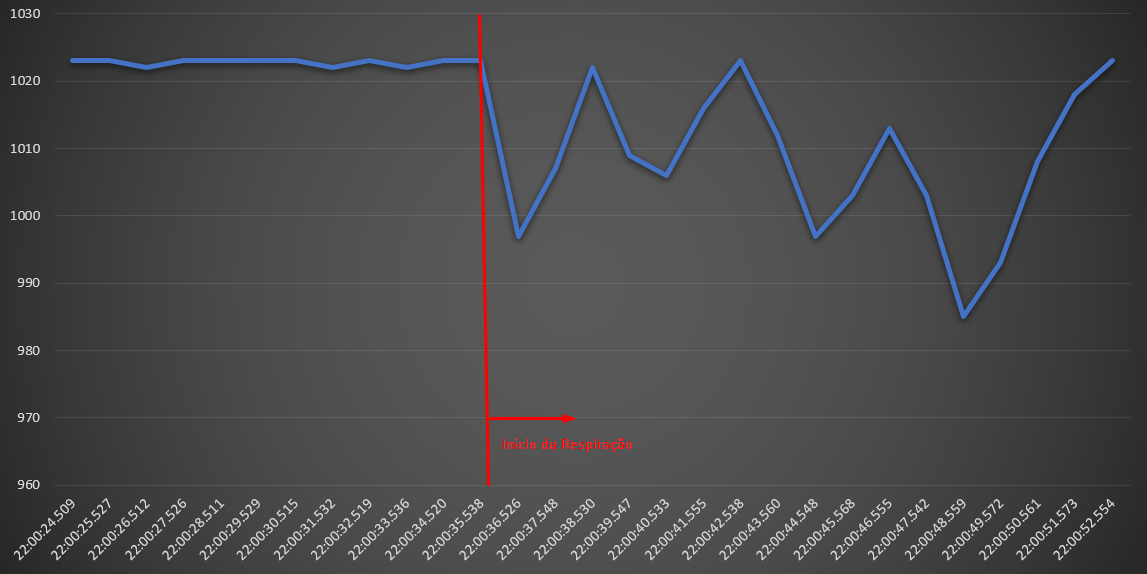
\includegraphics[width=1\linewidth]{images/RespostaCircuitoRealimentado.png}
		\caption{Resposta em curto prazo circuito realimentado (Tempo no eixo horizontal e valor de tensão quantizado no eixo vertical)}
		\label{fig:RespostaCircuitoRealimentado}
	\end{center}
\end{figure}

\begin{figure}[h!]
	\begin{center}
		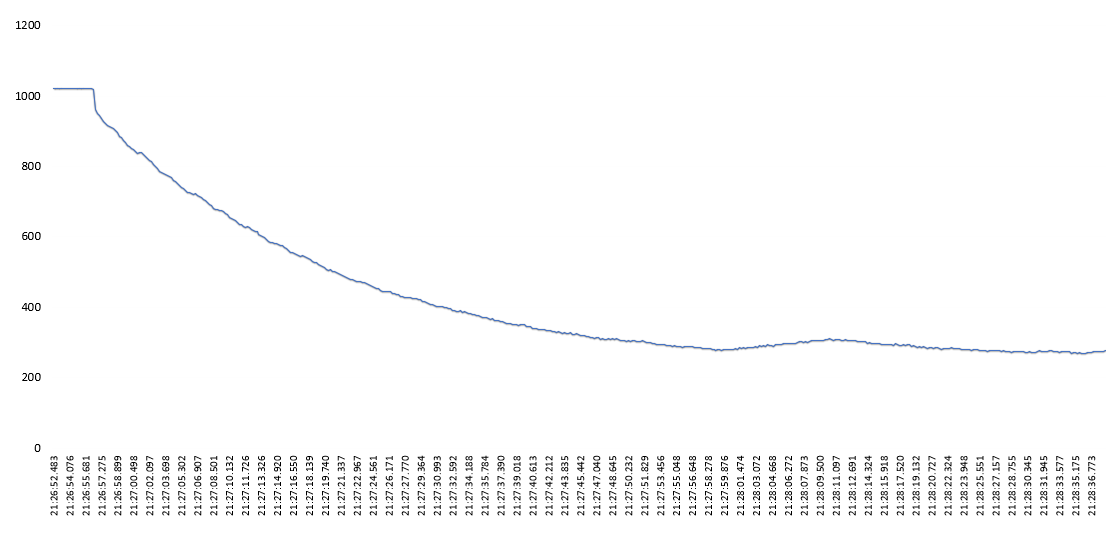
\includegraphics[width=1\linewidth]{images/DecaimentoRespiracaoMascara.png}
		\caption{Resposta de longo prazo circuito realimentado (Tempo no eixo horizontal e valor de tensão quantizado no eixo vertical)}
		\label{fig:RespostaCircuitoRealimentadoLongoPrazo}
	\end{center}
\end{figure}

\begin{figure}[h!]
	\begin{center}
		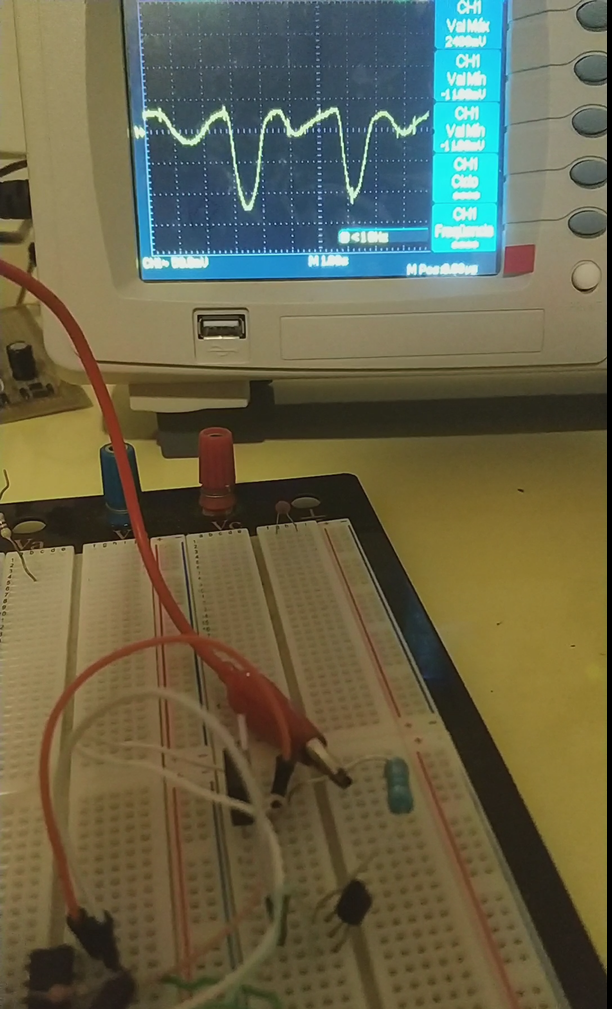
\includegraphics[width=1\linewidth]{images/sinal_osciloscopio.png}
		\caption{Sinal de saída do circuito realimentado no osciloscópio}
		\label{fig:sinal_osciloscopio}
	\end{center}
\end{figure}
\FloatBarrier


 
\section{O Software}

Em paralelo ao desenvolvimento do hardware, foi desenvolvido um software capaz de obter os dados de um microcontrolador através de uma porta serial no computador. Dada a escolha do Arduíno para o desenvolvimento do protótipo de baixo custo, era possível abstrair o desenvolvimento do hardware pressupondo, de antemão, que o circuito deveria ser projetado para entregar à entrada analógica do Arduíno um sinal de tensão variante entre $0V$ e $5V$. Para interpretar esse sinal, o microcontrolador existente no Arduíno (ATmega328) converte o sinal analógico em digital. A resolução do sinal convertido é dada pela equação \ref{eq:resolucaoArduino}, sendo o valor da tensão de referência igual a $5V$ e a quantidade de bits disponível para conversão igual a $10bits$, chegamos a uma resolução de $4,48mV$. Em outras palavras, abstraindo do hardware, o software deveria ser programado para ser capaz de receber uma entrada pela porta serial e ler sinais inteiros variando entre  $0$ e $1024$ (Equivalente a $10bits$) onde cada variação inteira representa $4,48mV$ do sinal de entrada do Arduíno.


\begin{equation} \label{eq:resolucaoArduino}
	Resolucao = \dfrac{V_{ref}}{2^n}
\end{equation}
Onde:
\begin{itemize}[label=]
	\item $V_{ref}$: Tensão de referência
	\item $n$: Número de bits do conversor
\end{itemize} 

A linguagem de programação escolhida para o desenvolvimento do software foi o Python dada a sua notória ascensão e eficiência para a realização de operações matemáticas e tratamento de dados científicos, além de ser referência em áreas como inteligência artificial (o que viabilizaria estudos futuros nessa área).

\subsection{Software de teste de conceitos} \label{sub:TesteDeConceitos}

\subsubsection{Leitura do sinal de entrada} \label{sub:LeituraSinalEntrada}


Antes de gerar um sinal simulado para iniciar o efetivamente o desenvolvimento do software, foi desenvolvido um pequeno protótipo para garantir que seria possível a comunicação entre um sinal gerado pelo Arduíno e o software desenvolvido em Python. Basicamente, existem dois softwares atuando simultaneamente para realizar essa leitura. Um, desenvolvido na linguagem de programação C, que fica instalado diretamente no Arduíno e é responsável por realizar a medição periódica e crua do sinal digital, logo após a sua quantização, e escrever um par valor x tempo na porta USB. O segundo é, de fato, o programa escrito em Python que, dentre outras funções realiza a leitura do sinal escrito pelo programa anterior na porta USB e salva os dados em um arquivo .csv, que poderá ser lido futuramente para a realização das operações matemáticas.


\begin{figure}[h!]
	\begin{center}
		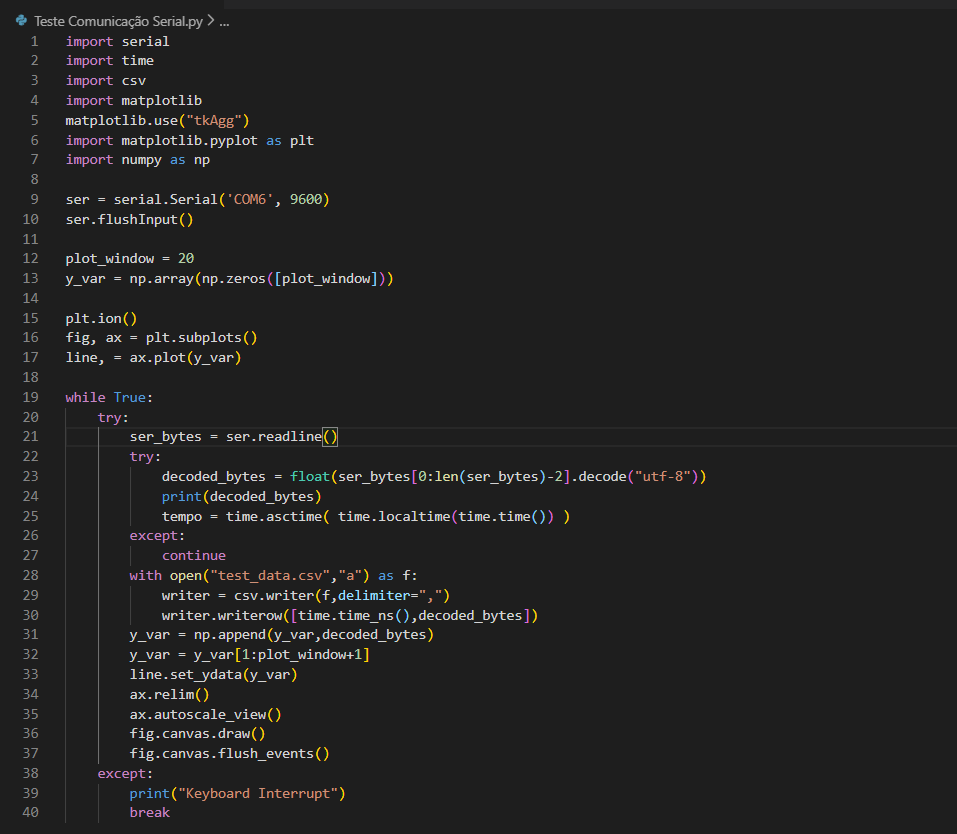
\includegraphics[width=1\linewidth]{images/LeitorDeUSB.png}
		\caption{Leitor de porta USB}
		\label{fig:LeitorDeUSB}
	\end{center}
\end{figure}


\subsubsection{Simulação do sinal de entrada}

Durante os experimentos com o hardware, foi possível observar um padrão na resposta do sinal analógico quando medido pelo osciloscópio que, em todas as versões do circuito, possuía um comportamento muito similar (imagem \ref{fig:sinal_osciloscopio}). A forma desse sinal pode ser explicada observando o princípio de funcionamento escolhido para que o sensor de temperatura seja capaz de medir a respiração. Em um cenário ideal, espera-se que o sensor esteja aquecido até que encontre uma temperatura de equilíbrio de operação e, quando em contato com um fluxo de ar da inspiração ou expiração, essa temperatura irá diminuir, aumentando a resistência do sensor e, em consequência, exibindo, no osciloscópio, uma diminuição da tensão. Quando acaba o fluxo de ar (tempo entre a expiração e inspiração), o circuito tentará esquentar novamente o sensor até que ele retorne à temperatura de equilíbrio. É possível também, observar que possuímos duas faixas distintas de amplitude na queda de tensão, o que nos faz concluir que o sensor tenderá a não obter uma resposta indiferente ao tipo de fluxo de ar (inspiração ou expiração) seja pelo fato de que a temperatura do ar na expiração é levemente maior, ou seja devido à construção que pode privilegiar o contato do fluxo do ar com o sensor em um sentido mais que no outro. Nos casos experimentados até então, por exemplo, a queda de tensão decorrente da inspiração era consideravelmente maior que a da expiração.


Considerando o comportamento dos sinais analógicos obtidos nas versões de circuito anteriores e o caráter cíclico natural do comportamento respiratório, o sinal de entrada foi simulado como um somatório de senoides com diferentes amplitudes e frequências. A frequência escolhida para o sinal principal foi a de 18 ciclos por minuto, que é a faixa superior da frequência considerada confortável para um adulto normal em repouso. Uma nova senoide com a metade da frequência foi gerada e posta defasada de modo a atenuar os picos referentes à expiração e agravar os relacionados à inspiração e, para a simulação do ruído, foi adicionada mais uma senoide com frequência mais elevada. O sinal simulado pode ser descrita conforme a equação \ref{eq:sinalSimulado} e produz o resultado apresentado no gráfico da figura \ref{fig:Funcao_simulada_interpolada}.

\begin{equation} \label{eq:sinalSimulado}
	F(t) =  \sin(0.15 * 2\pi t)  + 0.8\sin(\dfrac{\pi}{2} + 0.3 * 2\pi t) + 0.1\sin(\dfrac{\pi}{2} + 30 * 2\pi t)
\end{equation}


\begin{figure}[h!]
	\begin{center}
		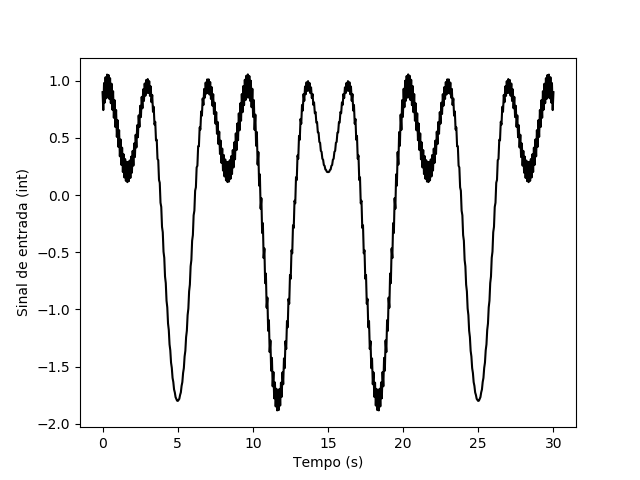
\includegraphics[width=0.5\linewidth]{images/Funcao_simulada_interpolada.png}
		\caption{Função simulada interpolada}
		\label{fig:Funcao_simulada_interpolada}
	\end{center}
\end{figure}



\subsubsection{Operações Realizadas}

A primeira versão do software foi projetada para ser capaz de realizar as seguintes operações:

\begin{itemize}[label=]
	\item 1- Ler os dados de uma porta serial via usb que serão enviados por um arduíno (trecho do código descrito na subseção \ref{sub:LeituraSinalEntrada})     
	\item     2- Criar pastas com o nome e horário das medições para o armazenamento dos arquivos
	\item     3- Salvar os dados em um arquivo .csv     
	\item     4- Ler os dados do arquivo csv e realizar as seguintes operações:     
	\subitem         4.1- Plotar diretamente
	\subitem         4.2- Plotar uma interpolação
	\subitem         4.3- Calcular a derivada primeira e segunda e plotar
	\subitem         4.4- Calcular a FFT e plotar    
	\item     5- Ler o arquivo csv, passar por um filtro IIR passa baixas, salvar um novo csv e realizar as seguintes operações:     
	\subitem         5.1- Plotar diretamente
	\subitem         5.2- Plotar uma interpolação
	\subitem         5.3- Calcular a derivada primeira e segunda e plotar
	\subitem         5.4- Calcular a FFT e plotar     
	\item     6- Ler o arquivo csv, passar por um filtro IIR passa baixas, salvar um novo csv e realizar as seguintes operações:        
	\subitem         6.1- Plotar diretamente
	\subitem         6.2- Plotar uma interpolação
	\subitem         6.3- Calcular a derivada primeira e segunda e plotar
	\subitem         6.4- Calcular a FFT e plotar     	 
\end{itemize} 

\subsubsection{Calculo das derivadas}

Para obter a derivada do sinal de entrada utilizamos o método das diferenças finitas \ref{eq:diferencasFinitas}, uma vez que, ao ser processado pelo programa, o sinal encontra-se discretizado e com uma boa quantidade de pontos devido a alta taxa de amostragem em relação à frequência de variação da tensão provocada pela respiração. O sinal discretizado é armazenado em dois vetores de mesmo tamanho, onde um armazena o valor da tensão e outro o valor do tempo de medição. Ao realizar o somatório da equação \ref{eq:diferencasFinitas} em todos os pontos dos vetores, conseguimos plotar o gráfico da derivada. Foi criada uma função no programa em Python que recebia como parâmetro os vetores x e y e retornava o resultado operação supracitada, permitindo assim o reuso do método para o cálculo da derivada segunda.


\begin{equation} \label{eq:diferencasFinitas}
	f'(x) =  \sum_{X0}^{Xn} \dfrac{f(x+\Delta x) - f(x)}{\Delta x}
\end{equation}
Onde:
\begin{itemize}[label=]
	\item $f'(x)$: Derivada da tensão no ponto x
	\item $X0$: Primeiro valor do vetor de tempo
	\item $Xn$: Último valor do vetor de tempo
	\item $f(x)$: Valor da tensão no ponto x
\end{itemize}

\subsubsection{Fast Fourier Transform (FFT)}

Para obter informações referentes à frequência do sinal respiratório, o sistema calcula e plota um gráfico realizando uma análise de Fourier, convertendo o sinal original, no domínio do tempo, em uma representação no domínio da frequência. Contudo,  realizar o cálculo da transformada de Fourier diretamente de sua definição \ref{eq:DTFT} implica em operações aritméticas de complexidade  \boldmath $O(n^2)$, entretanto, em meados da década de 1960, foi apresentado o algorítimo conhecido como transformada rápida de Fourier, ou FFT (Fast Fourier Transform),que pode ser encontrado nas anotações de Gauss \cite{heideman1985gauss}. Esse algorítimo mostrou-se perfeitamente adequado para uma eficiente implementação digital reduzindo em algumas ordens de grandeza o tempo necessário para calcular as transformadas \cite{oppenheim2010}. Em outras palavras, é possível obter o mesmo resultado da DTFT utilizando a FFT com uma complexidade de apenas $O(n \log (n)) $.   \unboldmath Aumentando assim a performance do software.



\begin{equation} \label{eq:DTFT}
	\mathcal{F} 	\left \{ f(t) \right \}  = \int_{-\infty}^{\infty} f(t) e^{-j \omega t}\,dt
\end{equation}

\subsubsection{Complexidade de algorítimo}

A complexidade de um algorítimo é determinada através da relação entre o tempo e memória gastos para realizar a operação de acordo com o tamanho da entrada. Ou seja, em termos práticos, é a complexidade do algorítimo, aliada à capacidade de processamento do computador, quem determinará a velocidade de funcionamento do sistema na medida em que se aumenta a quantidade de dados na entrada. Reduzir a complexidade de um algorítimo significa diminuir o tempo de execução do sistema.

A forma mais popular de representar a complexidade de tempo na análise de algorítimos é a \textbf{\textit{complexidade assintótica}}, que ignora fatores constantes e os termos que crescem mais lentamente. Por exemplo, em uma relação onde o tempo de execução $T(N)$ em função da entrada de dados $N$ é de $T(N) = 27N^2 + 45N + 12$, na medida em que $N$ aumenta, a função pode ser simplificada por $T(N) = 24N^2$. Simplificando ainda mais a análise, para prever o quão rápido será o crescimento do tempo de execução em relação ao aumento da entrada, podemos desconsiderar a constante que multiplica o termo de maior grau, uma vez que, tanto para $T(N) = 100000N^2$ quanto para $T(N) = 10N^2$, dobrar a entrada $N$ implicará em quadruplicar o tempo $T(N)$. Representamos $O(g)$ como sendo o limite superior para o tempo gasto por um algorítimo, em outras palavras, $O(g)$ representa a classe de funções que crescem, no máximo, tão rápidas quanto a função $g$. Ou seja, reduzir o cálculo da FFT de complexidade \boldmath $O(n^2)$ para $O(n \log (n)) $.   \unboldmath representa diminuir o tempo de execução, antes limitado pela função em vermelho, para a função em azul no gráfico da figura \ref{fig:grafico_complexidade}.

\begin{figure}[h!]
	\begin{center}
		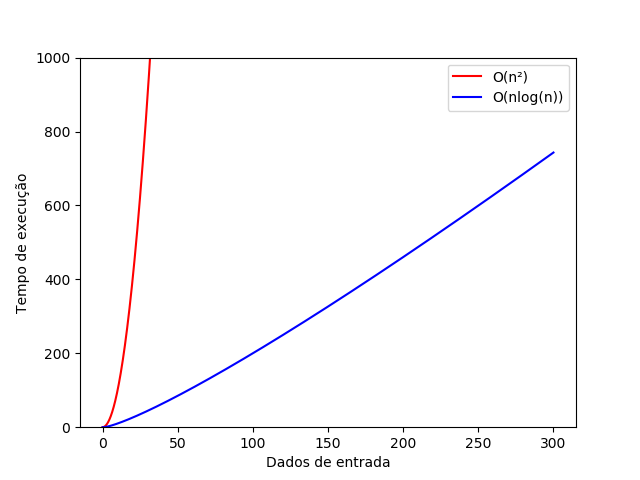
\includegraphics[width=0.7\linewidth]{images/Complexidade_algoritmo.png}
		\caption{Relação entre \boldmath $O(n^2)$ e $O(n \log (n)) $.   \unboldmath}
		\label{fig:grafico_complexidade}
	\end{center}
\end{figure}

\subsubsection{Filtro passa-baixas}

Com a finalidade de eliminar eventuais ruídos, o sistema é capaz de aplicar filtros passa-baixas digitais, eliminando altas frequências ruidosas e preservando as variações que ocorrem em uma faixa de frequência compatível com a respiração humana (abaixo de 70 ciclos por minuto em atletas). Os filtros digitais usam computação para implementar a ação de filtragem. Em comparação, existem duas classes de filtro digital \cite{haykin2001}, dependendo da sua resposta ao impulso (FIR e IIR) e, para maior liberdade do pesquisador, o sistema oferece as duas opções de filtragem.

\subsubsection{IIR (Infinite Impulse Response)}

Os filtros IIR são mais rápidos que os FIR. Para esse programa, foi escolhido o filtro de Butterworth, que possui resposta na frequência conforme a figura \ref{fig:Filtro_Butterworth}. Na medida em que aumentamos a ordem do filtro, conseguimos obter uma atenuação mais ingrime na filtragem \ref{fig:Ordem_Filtro_Butterworth}, contudo, adicionamos mais complexidade ao cálculo. Para o experimento, foi escolhida, empiricamente, o filtro de ordem 3. Chamamos de frequência de corte a frequência na qual o sinal possui atenuação de $-3 dB$ e esta foi escolhida de forma a permitir que o sinal na banda de frequências da respiração fosse preservado.

\begin{figure}[h!]
	\begin{center}
		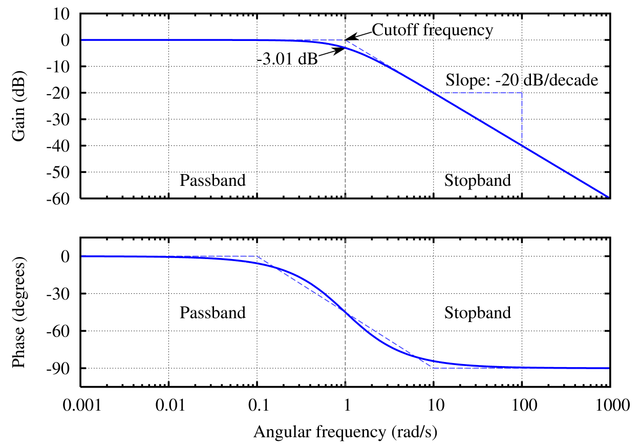
\includegraphics[width=0.7\linewidth]{images/Butterworth_filter_bode_plot.png}
		\caption{Resposta de um filtro Butterworth}
		\label{fig:Filtro_Butterworth}
	\end{center}
\end{figure}

\begin{figure}[h!]
	\begin{center}
		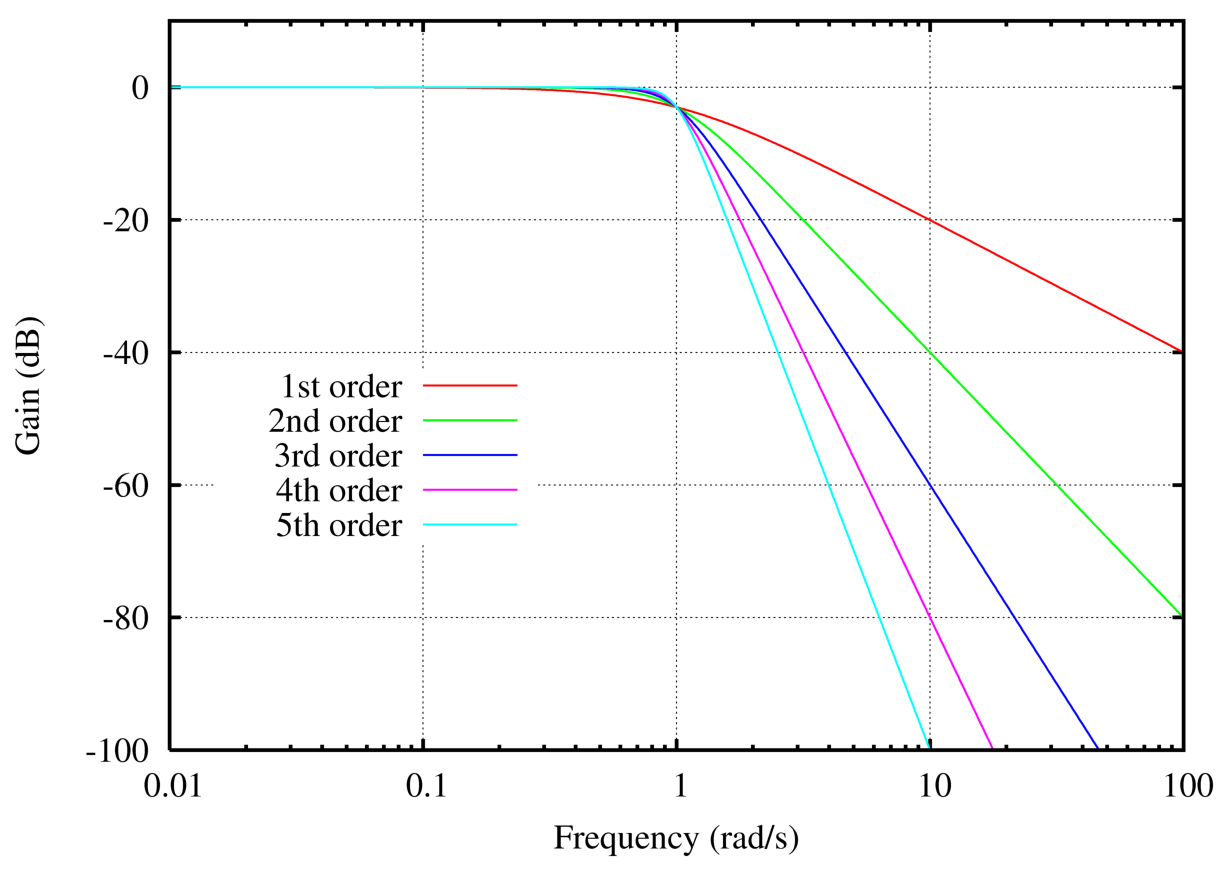
\includegraphics[width=0.5\linewidth]{images/Butterworth_orders.png}
		\caption{Resposta de um filtro Butterworth}
		\label{fig:Ordem_Filtro_Butterworth}
	\end{center}
\end{figure}

\subsubsection{FIR Finite Impulse Response}

A implementação do filtro FIR foi realizada utilizando o método de janelas. Nessa primeira fase do projeto, foi utilizada a janela de Hamming, que é definida pela equação \ref{eq:Hamming} e possui resposta em frequência conforme a figura \ref{fig:Janela_Hamming}.
 
 
\begin{equation} \label{eq:Hamming}
w(n) = 0,54 - 0,46\cos \left(\dfrac{2\pi n}{M - 1}\right) \qquad 0 \le n \le M-1
\end{equation} 

\begin{figure}[h!]
	\begin{center}
		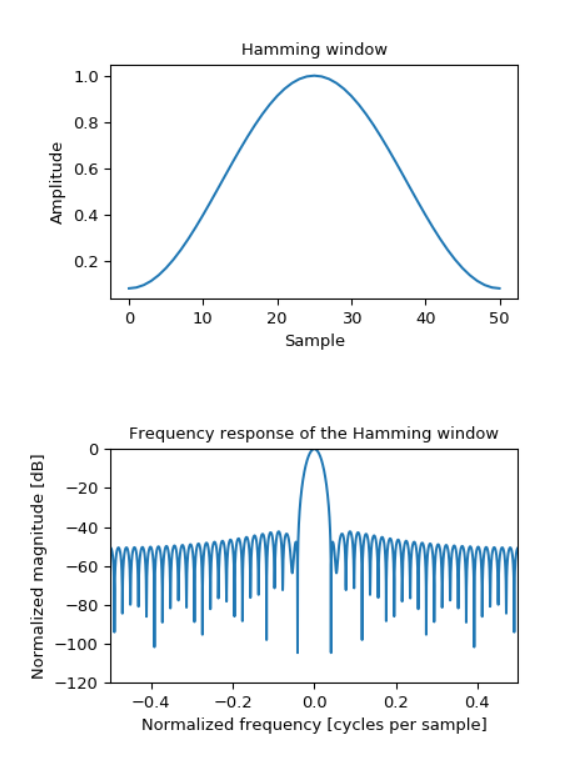
\includegraphics[width=1\linewidth]{images/janela_de_hamming.png}
		\caption{Resposta de uma janela de hamming}
		\label{fig:Janela_Hamming}
	\end{center}
\end{figure}

\subsection{Evolução do software para um sistema web}

Após validado o teste de conceitos, ou seja, após a certeza de que seria factível o desenvolvimento de uma aplicação capaz de ler os dados enviados pelo hardware através de uma porta usb, salvar em um arquivo .csv e realizar as operações matemáticas desejadas para a análise do sinal, foi desenvolvida uma aplicação web, gerando uma interface mais intuitiva e completa, que é capaz de armazenar dados referentes aos experimentos realizados, ao cadastro dos paciente, bem como as medições em um sistema de banco de dados, além de exibir os resultados em um gráfico interativo, com diversas funcionalidades, como aproximar, exportar, deslocar e etc. Com a finalidade de simplificar o uso da ferramenta, armazenar os dados de forma mais confiável e dar ao pesquisador uma melhor visualização dos dados e a possibilidade de exportar gráficos com melhor representação para ser usado em artigos científicos.O sistema é dividido em três telas, são elas: Tela principal (\ref{sec:tela_principal}), Tela de cadastro de pacientes (\ref{sec:tela_pacientes}) e Tela de cadastro de experimentos (\ref{sec:tela_experimentos}).

\subsubsection{Flask}

Desde o princípio do desenvolvimento do software, a linguagem escolhida para o processamento dos sinais foi o Python, por estar listada entre as melhores linguagens para o desenvolvimento de aplicações com inteligência artificial \cite{bestProgrammingLanguagesForAI2020}, sendo esse um campo em potencial para estudos futuros. Para o desenvolvimento de uma aplicação web utilizando o Python,  foi escolhido o Flask \cite{Flask} como framework, por aparentar ser um framework relativamente simples, suficiente para atender aos requisitos do sistema e com potencial escalável para desenvolvimentos futuros.

\subsubsection{MongoDB}

Atualmente, os bancos de dados são divididos em duas categorias, são elas:
\begin{itemize}[label=]
	\item - Banco de dados Relacionais.
	\item - Banco de dados não Relacionais.
\end{itemize}

Nos bancos de dados relacionais, os dados são armazenados em estruturas denominadas tabelas, onde cada tabela é composta por diversas colunas (atributos) e linhas (dados). Sua linguagem é o SQL (Structured Query Language). Essa categoria de banco de dados fornece uma estrutura consistente, porém rígida, onde cada entidade possui uma tabela e o relacionamento entre as entidades é realizado através de chaves primárias e chaves estrangeiras. Por exemplo, em uma aplicação onde são armazenadas informações na tabela "Paciente" conforme a figura \ref{fig:bd_relacional_antes}, os dados armazenados se apresentariam conforme o exemplo da figura \ref{fig:bd_relacional_dados}. Se o sistema que estiver utilizando esse modelo de dados precisar evoluir para uma estrutura que armazene as informações sobre endereço de forma mais detalhada, seria necessário criar uma nova tabela "Endereço" com novas colunas e alterar o tipo da coluna "endereço" da tabela "Paciente" para que esta não seja mais uma coluna que armazena o endereço, mas sim que armazene uma chave estrangeira apontando para a chave primária do endereço desejado, conforme as figuras \ref{fig:bd_relacional_intermediarios} e \ref{fig:bd_relacional_dados_depois}. Logo, nota-se que, em um cenário onde o sistema já possuía muitos pacientes com seus respectivos endereços cadastrados, seria necessário que cada endereço já existente fosse desmembrado e inserido nas colunas da tabela endereço, adicionando uma complexidade considerável na tentativa de evolução do sistema. Mais ainda, supomos que, em determinado momento, o sistema precise evoluir de maneira que um paciente possa cadastrar mais de um endereço. Em um banco relacional, seguindo a boa prática de modelagem de banco, seria necessário remover a coluna "endereço" da tabela "Paciente" e criar uma terceira tabela chamada "relPacienteEndereço", por exemplo, onde cada linha é responsável por relacionar pacientes e endereços (figuras \ref{fig:bd_relacional_final} e \ref{fig:bd_relacional_dados_finalpng}).


Portanto, para projetar um sistema que fosse maleável o suficiente e permitisse uma evolução fluida em projetos futuros, não era desejada a rigidez de um banco de dados relacional, sendo utilizado o banco não relacional. Nessa categoria, as informações são separadas em coleções e não possuem rigidez para seus atributos. Com o sistema construído com esse modelo de dados, se fosse necessário o mesmo processo evolutivo que descrevemos como exemplo para o banco de dados relacional, poderíamos, por exemplo manter os dados de endereço que já foram cadastrados na coleção paciente em um primeiro momento e, para os novos pacientes cadastrados na mesma coleção, armazenar um ou mais ids que apontam para a coleção Endereço (Conforme as figuras \ref{fig:bd_nao_relacional_Pacientes} e \ref{fig:bd_nao_relacional_Endereco}).

\begin{figure}[h!]
	\begin{center}
		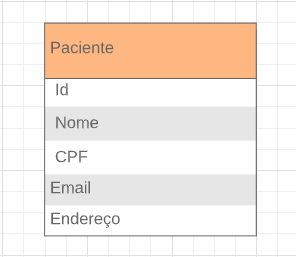
\includegraphics[width=0.2\linewidth]{images/bd_relacional_antes.png}
		\caption{Tabela Paciente banco relacional}
		\label{fig:bd_relacional_antes}
	\end{center}
\end{figure}

\begin{figure}[h!]
	\begin{center}
		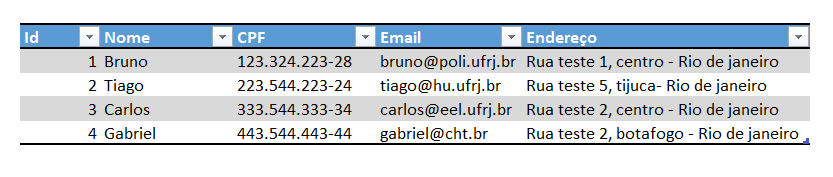
\includegraphics[width=1\linewidth]{images/bd_relacional_dados.png}
		\caption{Dados exemplo da tabela paciente}
		\label{fig:bd_relacional_dados}
	\end{center}
\end{figure}

\begin{figure}[h!]
	\begin{center}
		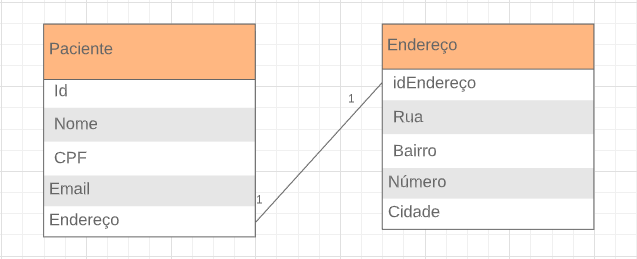
\includegraphics[width=0.3\linewidth]{images/bd_relacional_intermediario.png}
		\caption{Relacionamento paciente x endereço}
		\label{fig:bd_relacional_intermediarios}
	\end{center}
\end{figure}

\begin{figure}[h!]
	\begin{center}
		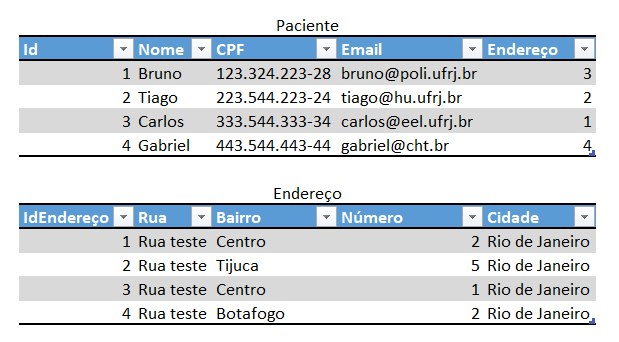
\includegraphics[width=0.8\linewidth]{images/bd_relacional_dados_depois.png}
		\caption{Dados exemplo das tabelas paciente e endereço}
		\label{fig:bd_relacional_dados_depois}
	\end{center}
\end{figure}

\begin{figure}[h!]
	\begin{center}
		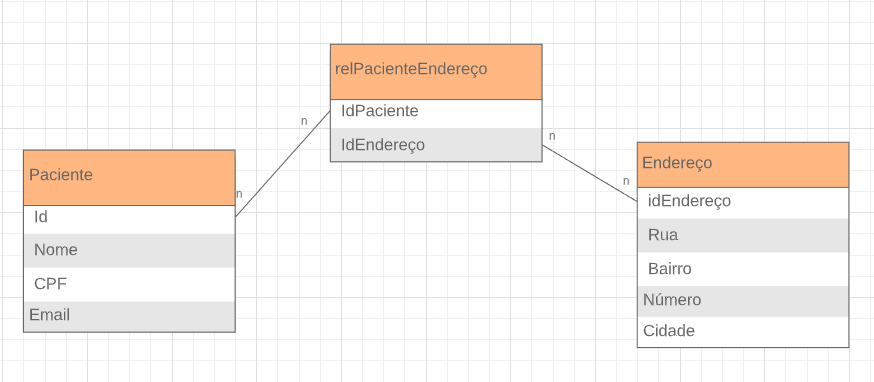
\includegraphics[width=0.3\linewidth]{images/bd_relacional_final.png}
		\caption{Relacionamento paciente x endereço}
		\label{fig:bd_relacional_final}
	\end{center}
\end{figure}

\begin{figure}[h!]
	\begin{center}
		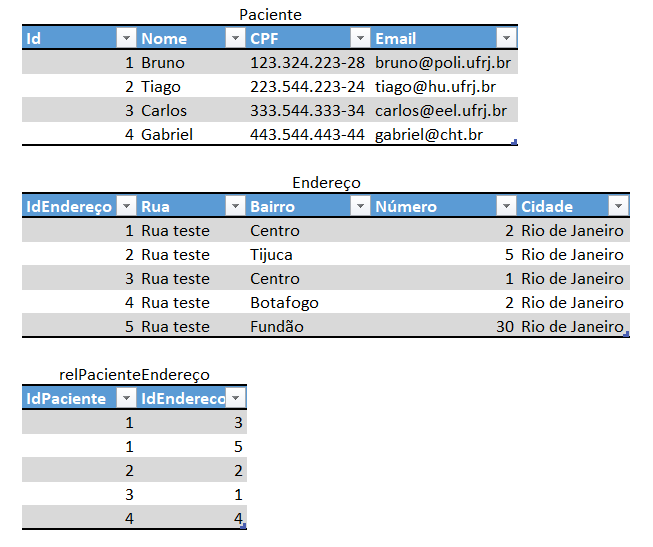
\includegraphics[width=0.8\linewidth]{images/bd_relacional_dados_finalpng.png}
		\caption{Dados exemplo das tabelas paciente e endereço}
		\label{fig:bd_relacional_dados_finalpng}
	\end{center}
\end{figure}

\begin{figure}[h!]
	\begin{center}
		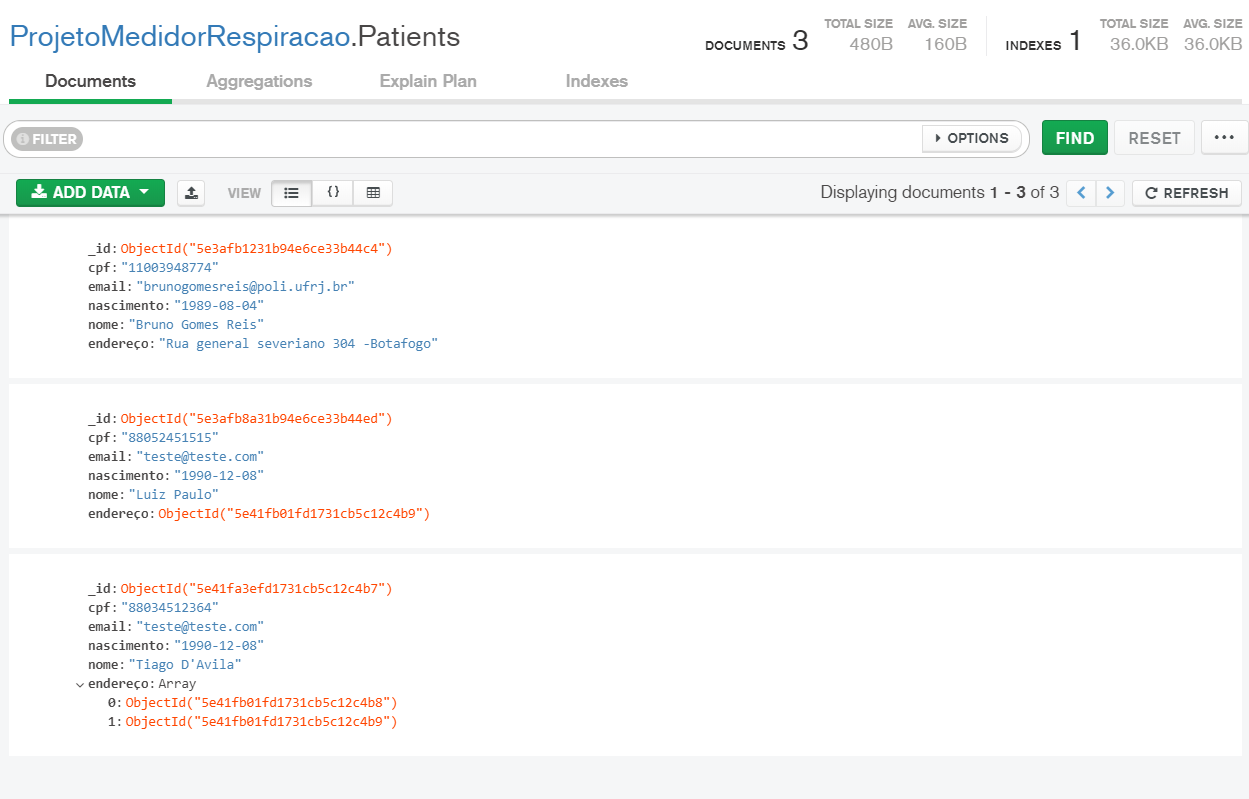
\includegraphics[width=0.8\linewidth]{images/bd_nao_relacional_Pacientes.png}
		\caption{Coleção "Paciente" no banco de dados não relacional}
		\label{fig:bd_nao_relacional_Pacientes}
	\end{center}
\end{figure}

\begin{figure}[h!]
	\begin{center}
		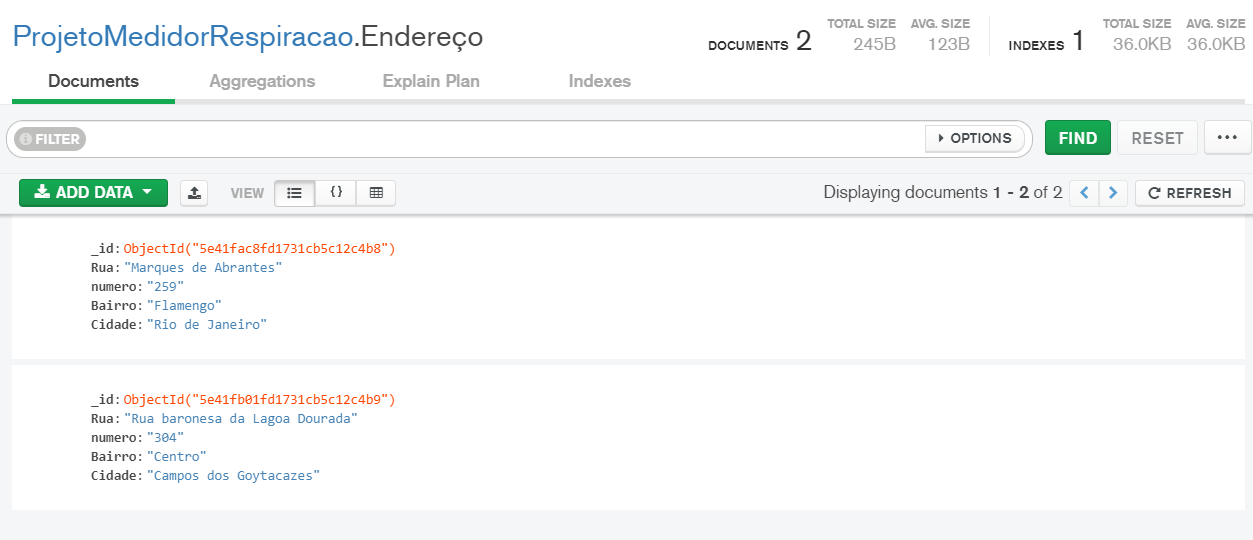
\includegraphics[width=0.8\linewidth]{images/bd_nao_relacional_Endereco.png}
		\caption{Coleção "Endereço" no banco de dados não relacional}
		\label{fig:bd_nao_relacional_Endereco}
	\end{center}
\end{figure}


Após a escolha do Flask como framework e do MongoDb (Banco de dados não relacional) como base de dados, foi desenvolvido o sistema web. Em seu menu superior é possível acessar 3 telas, são elas:

\begin{itemize}[label=]
	\item - Home
	\item - Cadastro
	\item - Experimento
\end{itemize}

\subsubsection{Tela de cadastro de Pacientes} \label{sec:tela_pacientes}

Ao selecionar a opção "Cadastro" no menu superior, o usuário é capaz de registrar um paciente, inserindo as informações "nome", "CPF", "E-mail" e "Data de Nascimento" (Figura \ref{fig:tela_cadastros}). Após preenchidas, se CPF inserido for um CPF válido, as informações são armazenadas no banco de dados (Figuras \ref{fig:paciente_salvo_tela} e \ref{fig:paciente_salvo_banco}). Caso contrário, o sistema exibe uma mensagem informando que trata-se de um CPF inválido (Figura \ref{fig:cpf_invalido_msg}). Para facilitar que o usuário observe a invalidade do CPF, o campo altera de cor dinamicamente, ficando verde caso o CPF seja válido e vermelho caso não seja (Figuras \ref{fig:cpf_invalido} e \ref{fig:cpf_valido}).


Para validar se trata-se de um CPF válido, o sistema foi desenvolvido utilizando um algorítimo fornecido pelo próprio ministério da fazenda, que consiste, basicamente, em operações utilizando os 9 primeiros dígitos e comparando o resultado dessas operações com os 2 últimos dígitos.

Utilizando, como exemplo, o CPF fictício 023.549.477-12

Validação do primeiro dígito:

Para validar o primeiro dígito, o sistema precisa multiplicar os 9 primeiros dígitos por uma sequência decrescente de 10 à 2. No nosso caso exemplo, teremos $0*10+2*9+3*8+5*7+4*6+9*5+4*4+7*3+7*2 = 197$ após realizada essa operação, o resultado deve ser multiplicado por $\dfrac{10}{11}$ e o resto dessa operação deve ser igual ao primeiro dígito da validação. No nosso caso $197*\dfrac{10}{11} =  \left \{ \begin{matrix} 179, & \mbox{Quociente} \\ 1, & \mbox{Resto}\end{matrix} \right.	$, portanto, o resto está igual ao primeiro dígito dos últimos 2 dígitos de validação.

Validação do segundo dígito:

Passada a validação do primeiro dígito, para que o cpf seja válido, é necessário validar o segundo dígito. Para isso, o sistema precisa utilizar os 9 primeiros dígitos e o primeiro dígito da validação em uma operação similar à realizada na primeira verificação. Todos os números são multiplicados por uma escala que vai de 11 à 2 de acordo com sua posição. Sendo assim, para o nosso exemplo, teremos $0*11+2*10+3*9+5*8+4*7+9*6+4*5+7*4+7*3+1*2 = 240$ e $240*\dfrac{10}{11} =  \left \{ \begin{matrix} 218, & \mbox{Quociente} \\ 2, & \mbox{Resto}\end{matrix} \right.	$. Sendo o resto igual ao último dígito de validação, o CPF está eleito para ser um CPF válido.

Números inválidos conhecidos

Além das operações de validação dos primeiro e segundo dígito, o algorítimo elimina alguns casos de CPFs inválidos conhecidos que podem furar as regras de validação, como é o caso dos CPFs com números repetidos (Ex: 111.111.111-11).


\begin{figure}[h!]
	\begin{center}
		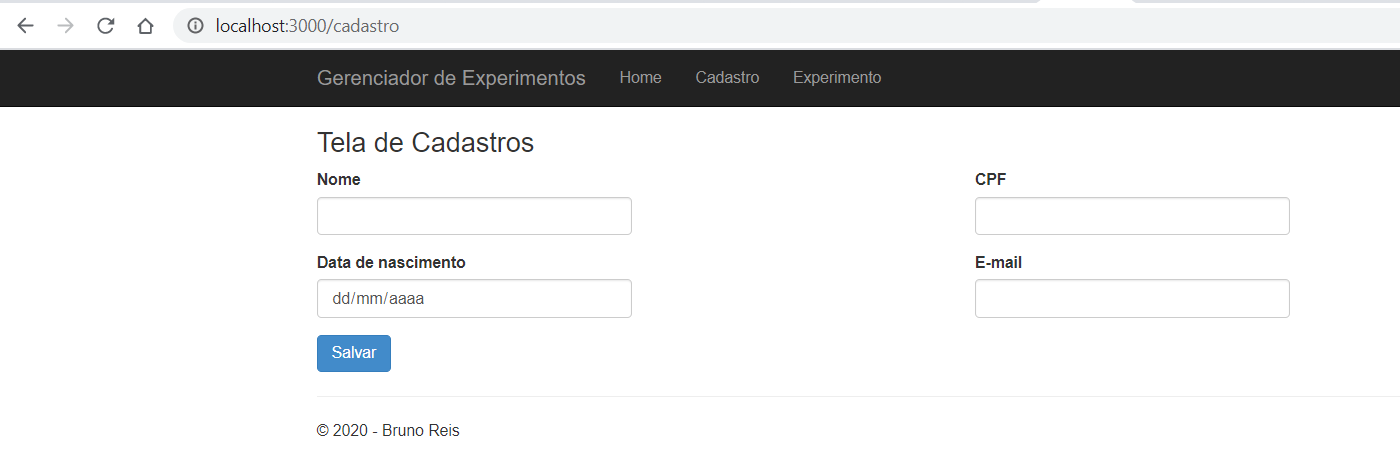
\includegraphics[width=0.8\linewidth]{images/tela_cadastros.png}
		\caption{Tela de Cadastros}
		\label{fig:tela_cadastros}
	\end{center}
\end{figure}

 \begin{figure}[h!]
 	\begin{center}
 		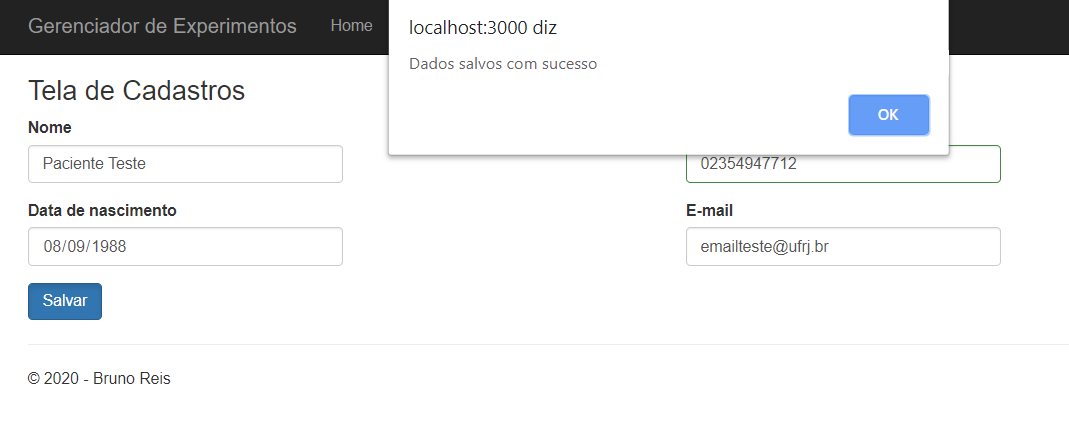
\includegraphics[width=0.8\linewidth]{images/paciente_salvo_tela.png}
 		\caption{Paciente Salvo}
 		\label{fig:paciente_salvo_tela}
 	\end{center}
 \end{figure}
 
 \begin{figure}[h!]
 	\begin{center}
 		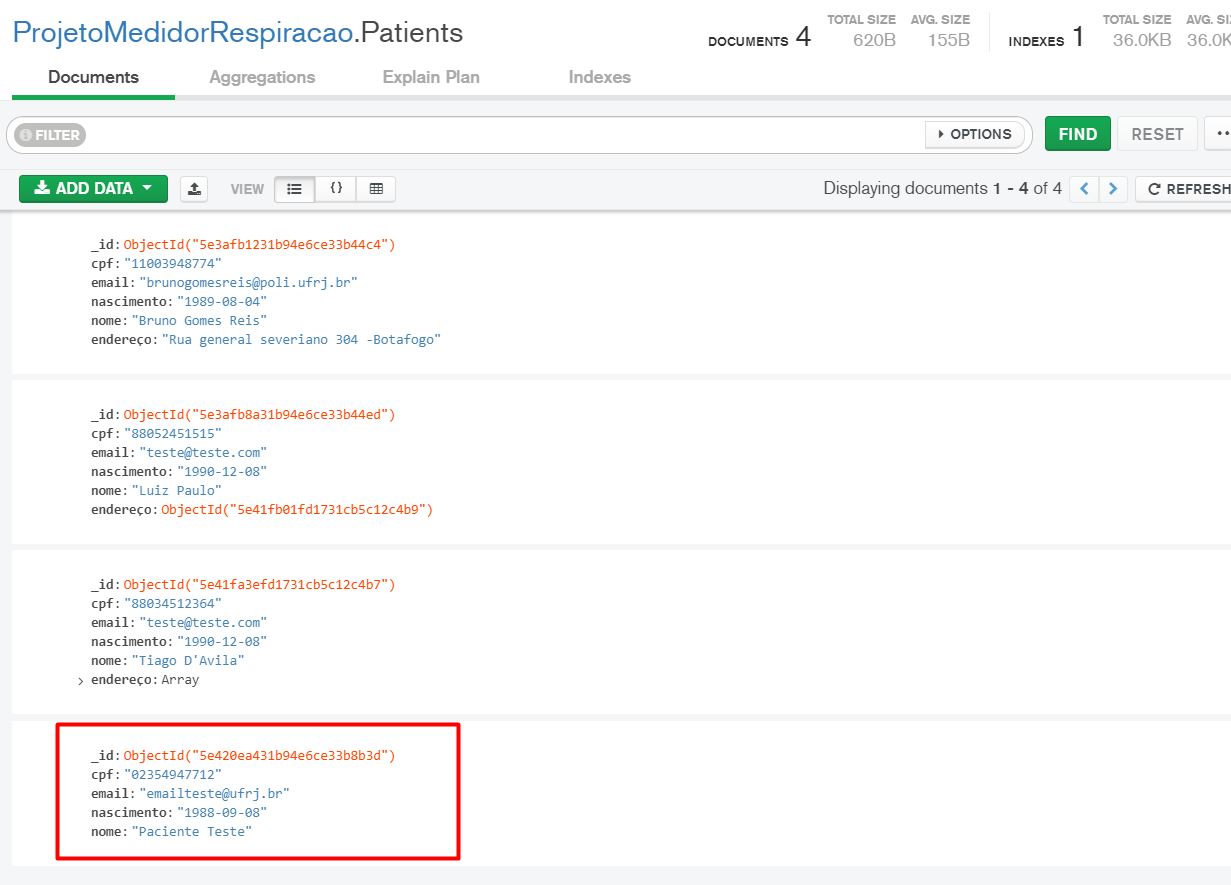
\includegraphics[width=0.8\linewidth]{images/paciente_salvo_banco.png}
 		\caption{Paciente Salvo no Banco de Dados}
 		\label{fig:paciente_salvo_banco}
 	\end{center}
 \end{figure}
 
  \begin{figure}[h!]
 	\begin{center}
 		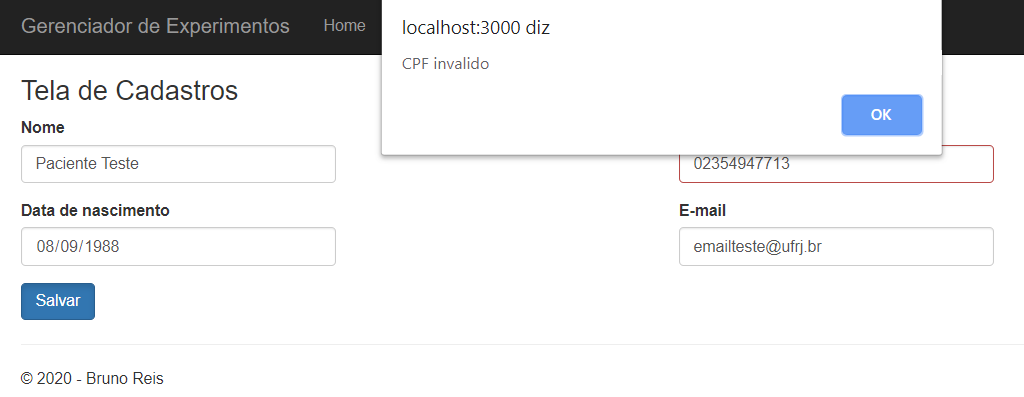
\includegraphics[width=0.8\linewidth]{images/cpf_invalido_msg.png}
 		\caption{Mensagem de Erro ao salvar Paciente}
 		\label{fig:cpf_invalido_msg}
 	\end{center}
 \end{figure}

  \begin{figure}[h!]
	\begin{center}
		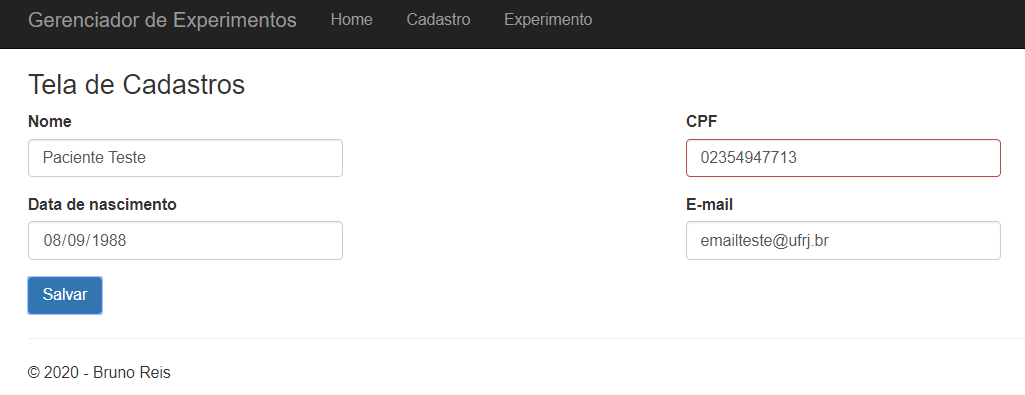
\includegraphics[width=0.8\linewidth]{images/cpf_invalido.png}
		\caption{Campo com CPF inválido}
		\label{fig:cpf_invalido}
	\end{center}
\end{figure}

  \begin{figure}[h!]
	\begin{center}
		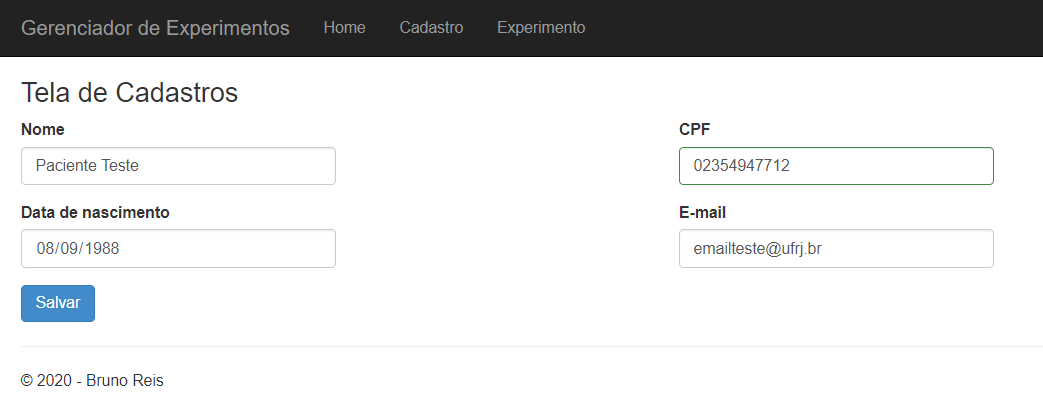
\includegraphics[width=0.8\linewidth]{images/cpf_valido.png}
		\caption{Campo com CPF válido}
		\label{fig:cpf_valido}
	\end{center}
\end{figure}

\subsubsection{Tela de Experimentos} \label{sec:tela_experimentos}

Ao acionar a opção "Experimento" no menu superior, o usuário é capaz é direcionado para uma tela (Figura \ref{fig:experimento}) em que pode escolher um experimento já cadastrado (Figura \ref{fig:experimento_lista}) ou cadastrar um novo experimento, além de associar pacientes já cadastrados e fazer o upload de arquivos .csv, que podem conter os dados obtidos pelo hardware \ref{sub:LeituraSinalEntrada} ou dados de qualquer outra origem, desde que estejam divididos com o eixo x na primeira coluna e o eixo y na segunda coluna, ambas com cabeçalho e começando a inserção dos dados na linha 2. Ao acionar o botão de upload, o sistema abre uma janela para que o usuário procure e adicione o arquivo .csv armazenado em seu computador local (Figura \ref{fig:experimento_csv}).


  \begin{figure}[h!]
	\begin{center}
		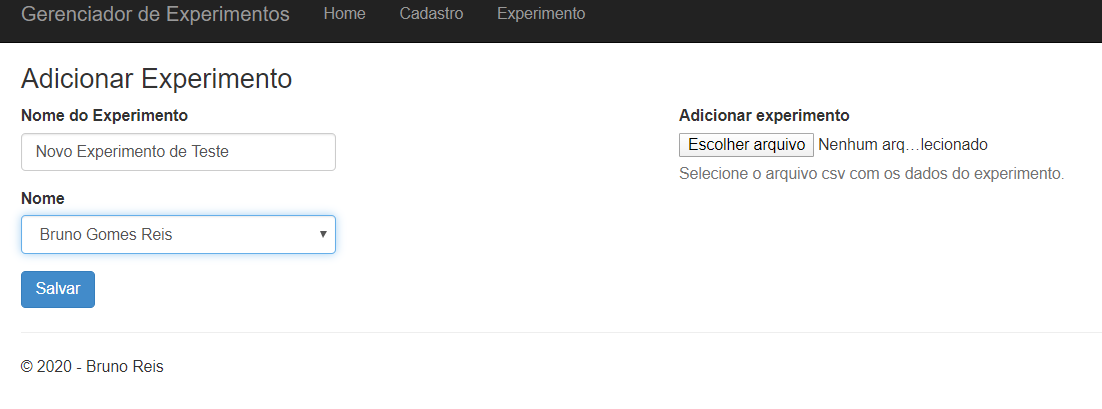
\includegraphics[width=0.8\linewidth]{images/experimento.png}
		\caption{Tela de Experimento}
		\label{fig:experimento}
	\end{center}
\end{figure}

  \begin{figure}[h!]
	\begin{center}
		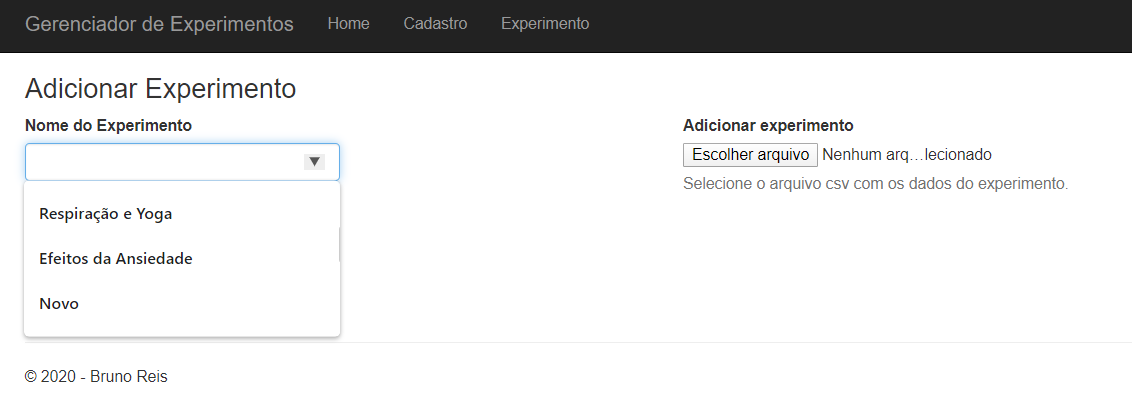
\includegraphics[width=0.8\linewidth]{images/experimento_lista.png}
		\caption{Lista de experimentos existentes no banco de dados}
		\label{fig:experimento_lista}
	\end{center}
\end{figure}

  \begin{figure}[h!]
	\begin{center}
		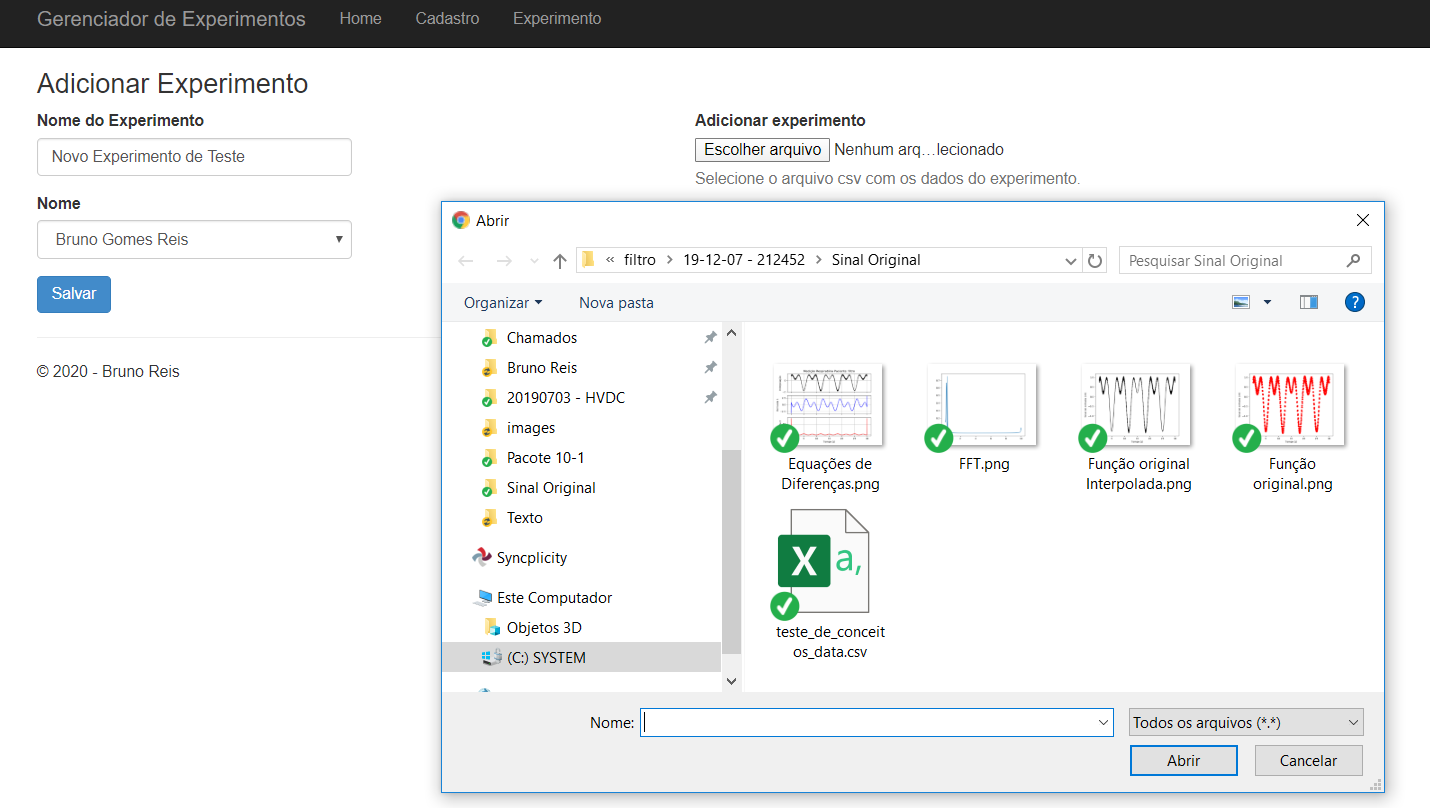
\includegraphics[width=0.8\linewidth]{images/experimento_csv.png}
		\caption{Tela para upload de arquivo .csv}
		\label{fig:experimento_csv}
	\end{center}
\end{figure}


\subsubsection{Tela Principal} \label{sec:tela_principal}

Ao acessar a página principal, ou ao selecionar a opção "Home" no menu principal, o sistema irá exibir a tela da figura \ref{fig:home}. Nessa tela, será exibido um gráfico aleatório e os campos "Experimento" e "Paciente" não estarão preenchidos. Ao apertar em algum desses campos, será exibido um modal \ref{fig:home_lista} com a lista de experimentos ou pacientes cadastrados para que o usuário possa selecionar qual medição ele deseja analisar. Ao escolher o experimento e o paciente desejado, o usuário pode utilizar qualquer um dos 4 botões localizados na parte inferior da tela para escolher qual análise quer exibir. As opções são:

\begin{itemize}
	\item - Sinal quantizado
	\item - Sinal interpolado
	\item - Análise de Fourier
	\item - Equação de diferenças
\end{itemize}

Ao posicionar o mouse em cima dos botões "Equação de Diferenças" e "Análise de fourier" é exibido um aviso com as respectivas formulas (Fuguras \ref{fig:home_diferencas} e \ref{fig:home_fourier}) 

É possível também encontrar no canto superior direito uma lista contendo os filtros possíveis de serem utilizados:

\begin{itemize}
	\item FiltroOriginal
	\item Filtro IIR
	\item Filtro FIR
\end{itemize}

Todas as operações matemáticas realizadas foram descritas na seção \ref{sub:TesteDeConceitos}.


  \begin{figure}[h!]
	\begin{center}
		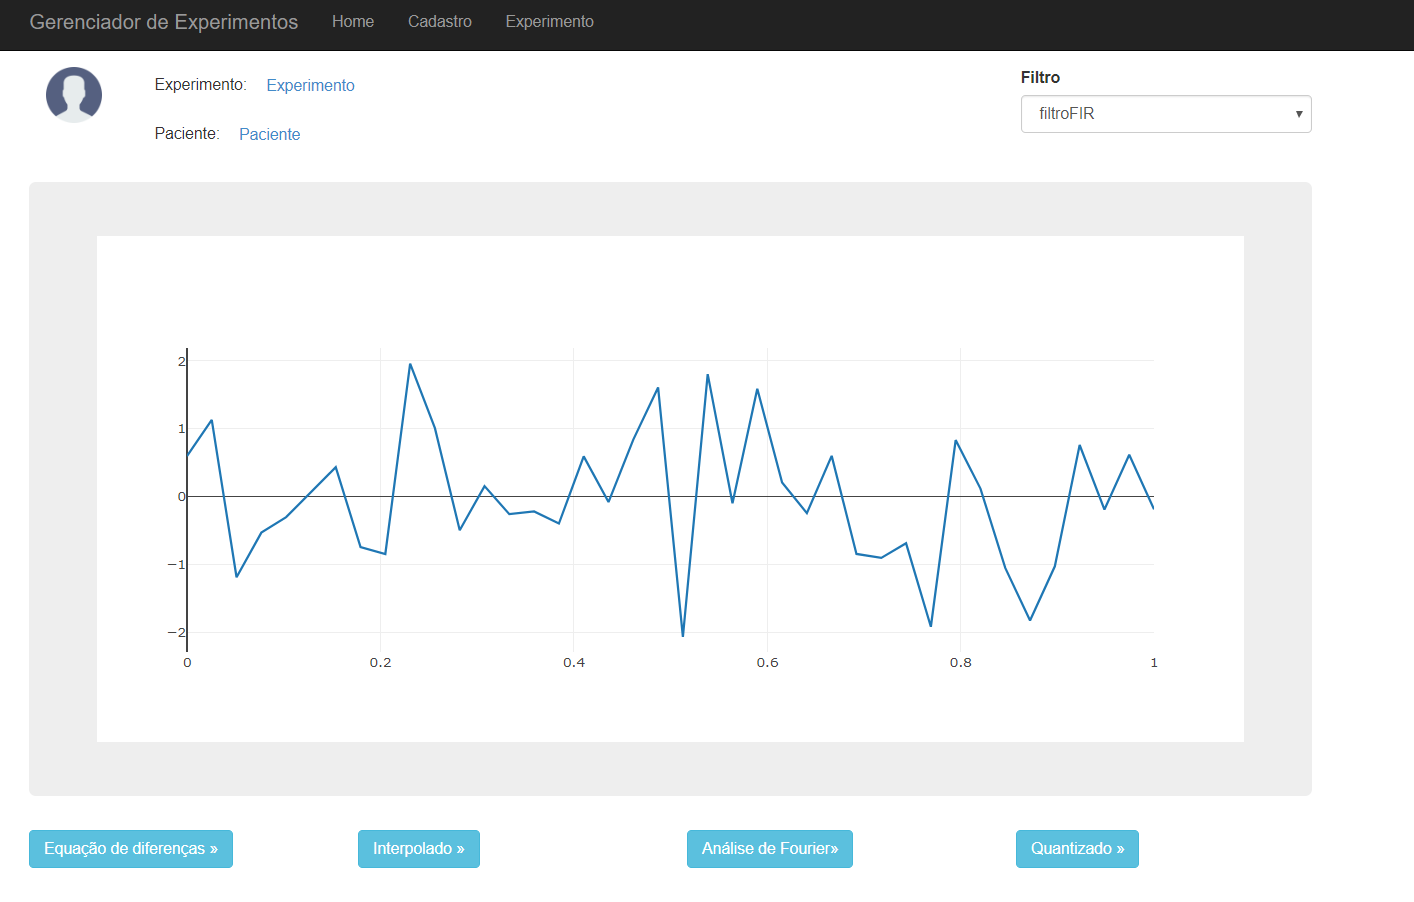
\includegraphics[width=0.8\linewidth]{images/home.png}
		\caption{Tela Principal}
		\label{fig:home}
	\end{center}
\end{figure}

  \begin{figure}[h!]
	\begin{center}
		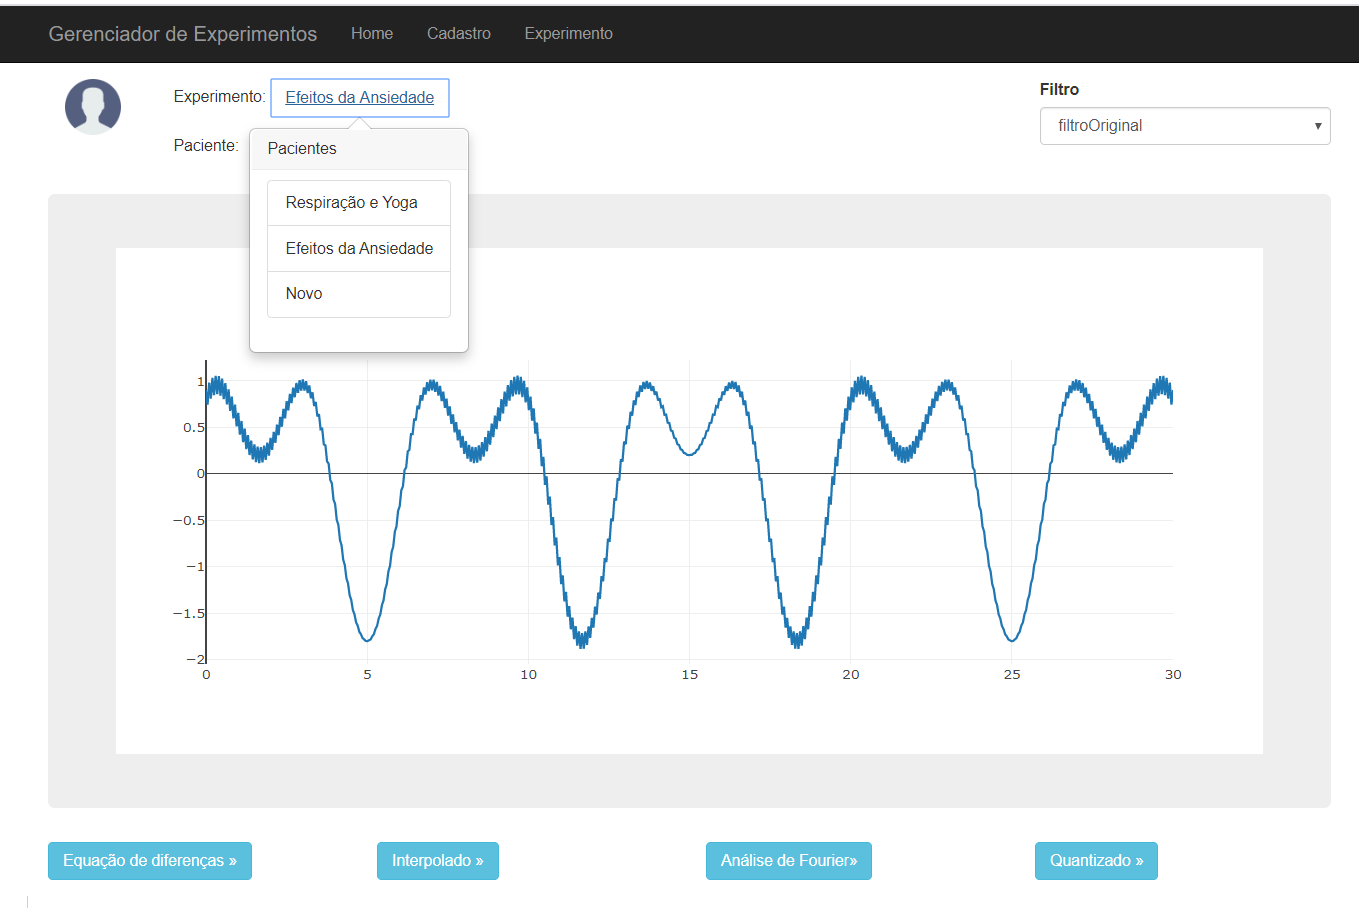
\includegraphics[width=0.8\linewidth]{images/home_lista.png}
		\caption{Tela Principal}
		\label{fig:home_lista}
	\end{center}
\end{figure}

\begin{figure}[h!]
	\begin{center}
		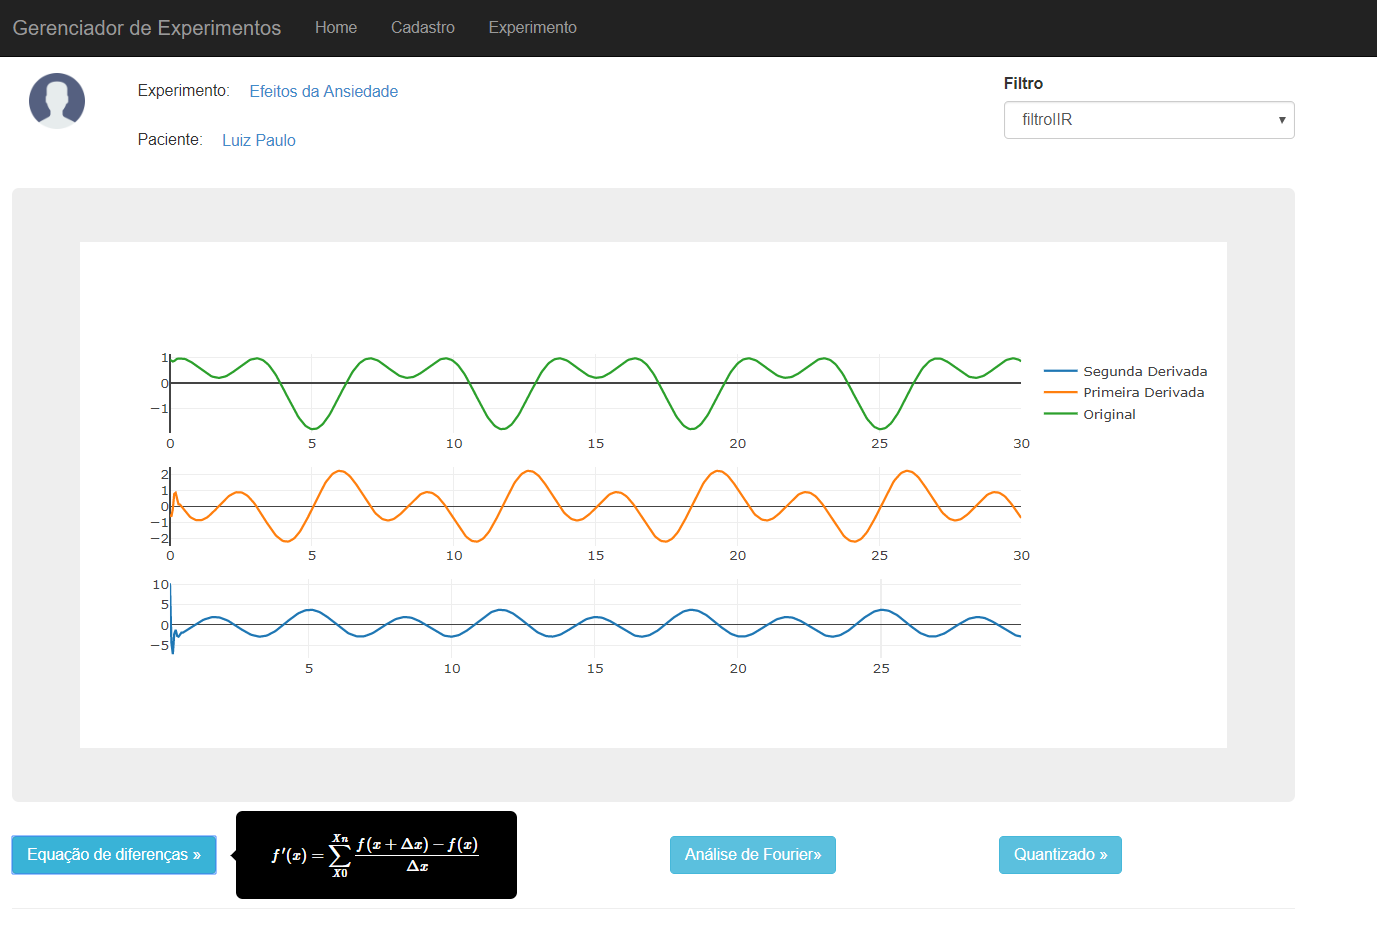
\includegraphics[width=0.8\linewidth]{images/home_diferencas.png}
		\caption{Equação de diferenças}
		\label{fig:home_diferencas}
	\end{center}
\end{figure}

\begin{figure}[h!]
	\begin{center}
		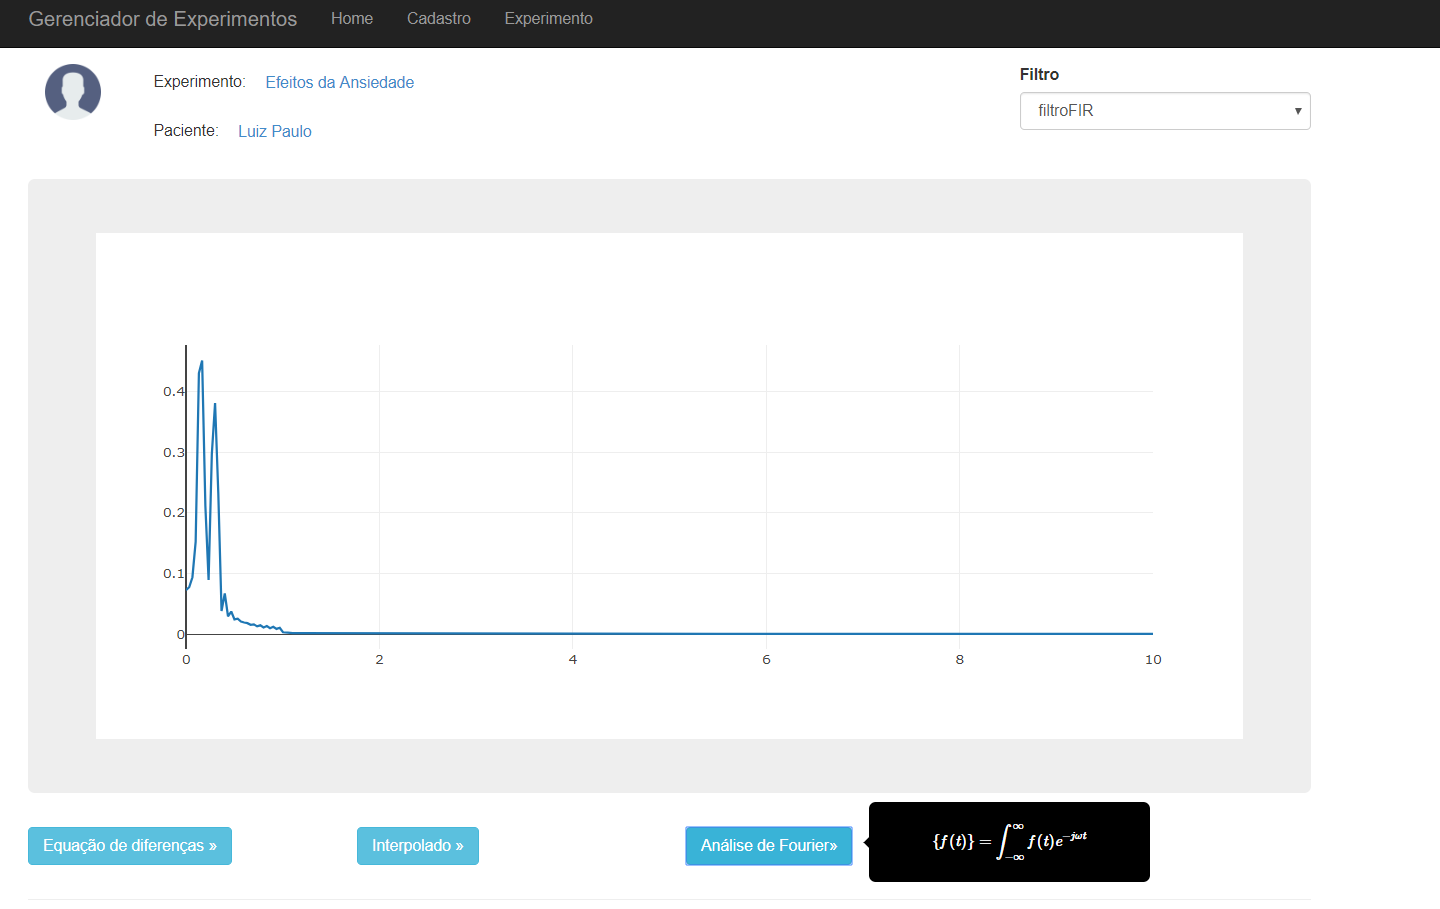
\includegraphics[width=0.8\linewidth]{images/home_fourier.png}
		\caption{Análise de Fourier}
		\label{fig:home_fourier}
	\end{center}
\end{figure}

Para facilitar a visualização dos dados, o sistema exibe o valor dos eixos ao posicionar o mouse em cima do local desejado no gráfico (\ref{fig:home_posicao_mouse}) e, caso necessário, o usuário pode arrastar a tela com o mouse dando um zoom na região desejada (Figuras \ref{fig:home_zoom_mouse} e \ref{fig:home_zoom_mouse2}).

\begin{figure}[h!]
	\begin{center}
		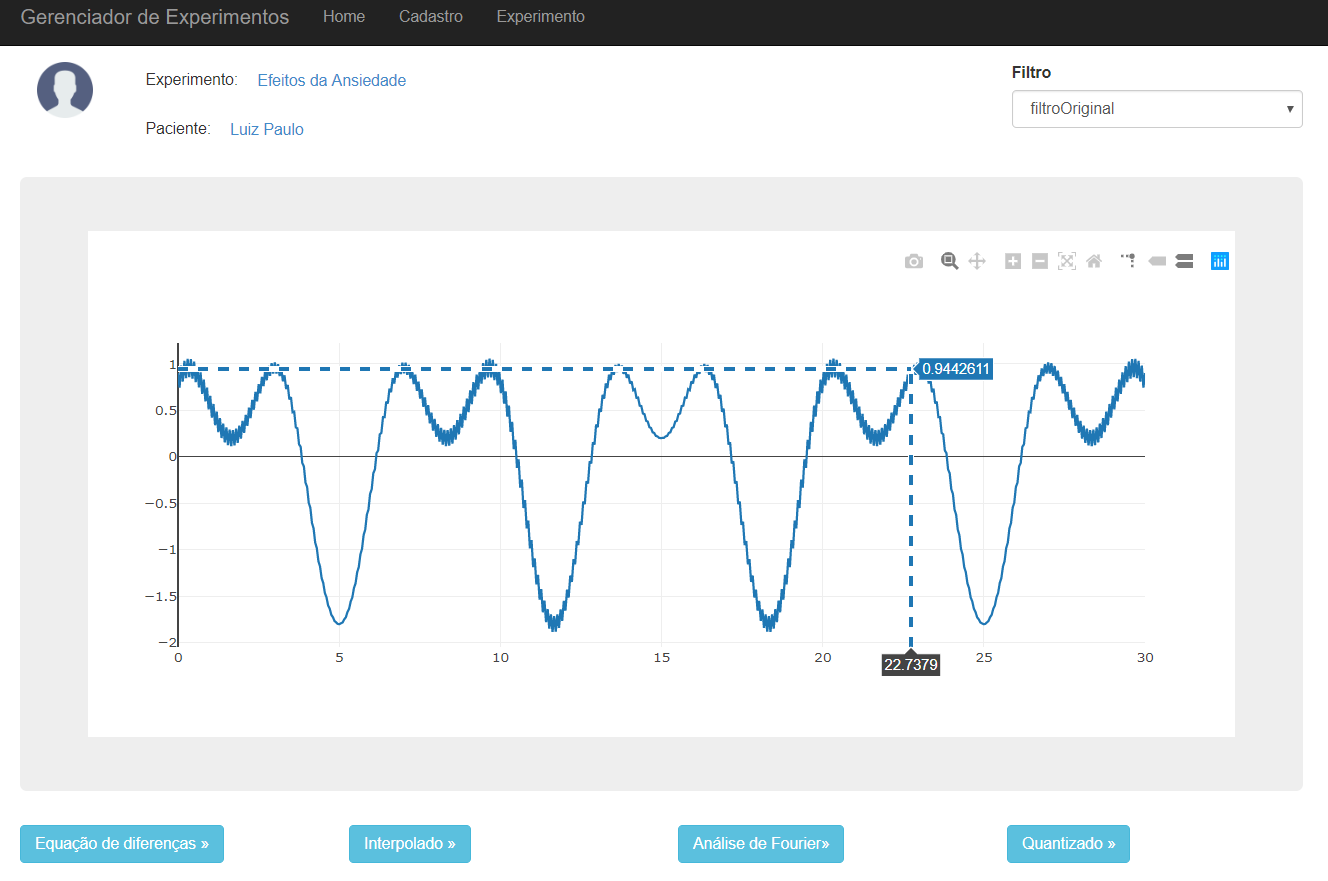
\includegraphics[width=0.8\linewidth]{images/home_posicao_mouse.png}
		\caption{Exibindo valor do ponto no gráfico}
		\label{fig:home_posicao_mouse}
	\end{center}
\end{figure}

\begin{figure}[h!]
	\begin{center}
		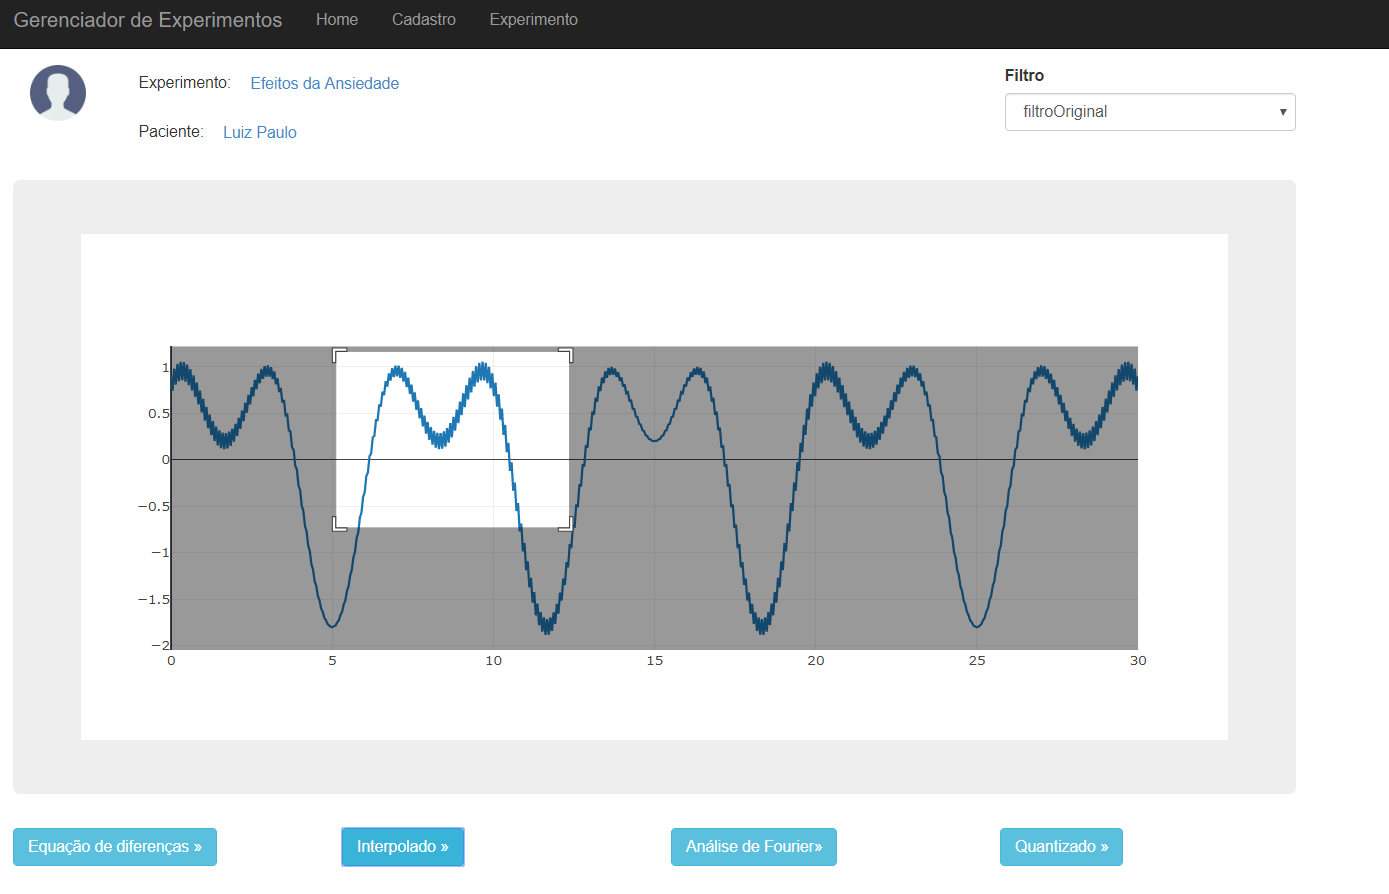
\includegraphics[width=0.8\linewidth]{images/home_zoom_mouse.png}
		\caption{Selecionando área do gráfico desejada}
		\label{fig:home_zoom_mouse}
	\end{center}
\end{figure}

\begin{figure}[h!]
	\begin{center}
		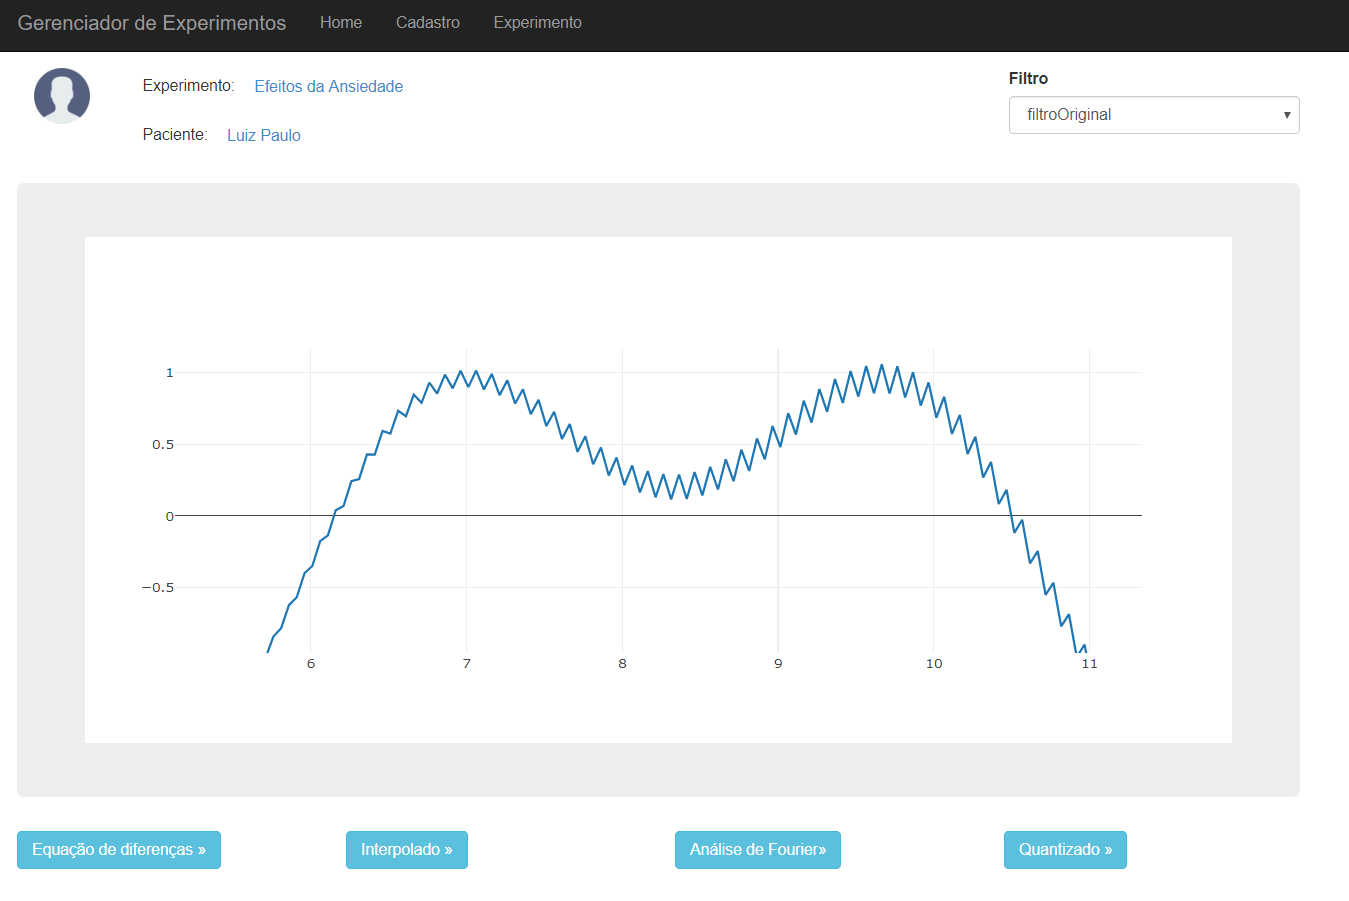
\includegraphics[width=0.8\linewidth]{images/home_zoom_mouse2.png}
		\caption{zoom na área selecionada}
		\label{fig:home_zoom_mouse2}
	\end{center}
\end{figure}

Por fim, existem algumas funcionalidades úteis no canto superior direito do gráfico, que permitem ao usuário dar zoom in, zoom out, fazer download do gráfico, deslocar o gráfico para esquerda ou direita, exibir linhas no eixo x e y e retornar a escala para o valor original. 